
\chapter{Resultados}
\section{Identificación de propuestas regioquímicas}

Para determinar la viabilidad termodinámica y la reactividad de la primera adición de glicina sobre la jaula del $\text{C}_{60}$, se llevaron a cabo cálculos de optimización de geometría y análisis de frecuencias vibracionales empleando la Teoría de Funcionales de la Densidad (DFT) con el funcional híbrido B3LYP y el conjunto de bases 6-311G(d,p). La ausencia de frecuencias imaginarias en los  cálculos confirmó que todas las estructuras corresponden a mínimos locales en la superficie de energía potencial. Adicionalmente, se determinaron las funciones de Fukui para evaluar la reactividad electrofílica y nucleofílica local de la jaula.

Debido a la alta simetría icosaédrica ($I_h$) del $\text{C}_{60}$ prístino, los 60 átomos de carbono son químicamente equivalentes previo a la reacción. Por lo tanto, en todas las propuestas evaluadas la molécula de glicina se ancló sobre el carbono C59, variando la posición de adición del átomo de hidrógeno complementario para mapear la regioquímica del sistema (Figura~\ref{fig:isomeros-gly1}):

\begin{itemize}
    \item \textbf{Isómero $\text{C}_{60}(\text{Gly})$-a (C59, C43):} El átomo de hidrógeno se localiza en una posición frontal sobre la cara del pentágono con respecto al grupo glicina.
    \item \textbf{Isómero $\text{C}_{60}(\text{Gly})$-b (C59, C58):} Representa una disposición de adición en posición \textit{para} en la red hexagonal contigua con respecto a la glicina.
    \item \textbf{Isómero $\text{C}_{60}(\text{Gly})$-c (C59, C11):} Corresponde a una adición vicinal (1,2) en posición \textit{orto} a través de un enlace de tipo [6,6] (fusión hexágono-hexágono).
    \item \textbf{Isómero $\text{C}_{60}(\text{Gly})$-d (C59, C10):} Constituye una adición vicinal (1,2) a través de un enlace de tipo [5,6] (fusión pentágono-hexágono) entre los carbonos C59 y C10.
    \item \textbf{Isómero $\text{C}_{60}(\text{Gly})$-e (C59, C50):} Propuesta diseñada en una región opuesta (antípoda) de la jaula con el fin de evaluar y descartar si las interacciones a larga distancia o la polarización de la red generan una mayor estabilidad termodinámica.
    \item \textbf{Isómero $\text{C}_{60}(\text{Gly})$-f (C59, C51):} Corresponde a la funcionalización en un carbono adyacente a la posición opuesta evaluada en el inciso (e).
\end{itemize}

\begin{table}[H]
    \centering
    \caption{Energías de formación de los isómeros del complejo $C_{60}(\text{Gly})$.}
    \label{tab:isomeros-gly1}
    \renewcommand{\arraystretch}{1.15}
    \begin{tabular}{lcc}
        \toprule
        \textbf{Isómero} & \textbf{Carbonos de enlace} & \textbf{Energía relativa (kcal mol$^{-1}$)} \\
        \midrule
      C\textsubscript{60}(Gly)-a & C59, C43 & 0.059 \\
      C\textsubscript{60}(Gly)-b & C59, C58 & 0.010 \\
         C\textsubscript{60}(Gly)-c & C59, C11 & 0.000 \\
         C\textsubscript{60}(Gly)-d & C59, C10 & 0.027 \\
        C\textsubscript{60}(Gly) -e & C59, C50 & 0.074 \\
         C\textsubscript{60}(Gly)-f & C59, C51 & 0.045 \\
        \bottomrule
    \end{tabular}
\end{table}

\subsubsection{Análisis de energías relativas y control de reacción}

Los resultados energéticos recopilados en la Tabla~\ref{tab:isomeros-gly1} muestran que las energías relativas de formación oscilan en un rango extremadamente estrecho, desde $0.000\text{ kcal mol}^{-1}$ ($\text{C}_{60}(\text{Gly})$-c) hasta $-0.074\text{ kcal mol}^{-1}$ ($\text{C}_{60}(\text{Gly})$-e). Desde el punto de vista de la fisicoquímica teórica, diferencias energéticas inferiores a $0.1\text{ kcal mol}^{-1}$ se encuentran significativamente por debajo del margen de error numérico del funcional B3LYP (típicamente $1\text{--}2\text{ kcal mol}^{-1}$) y de la energía térmica ambiental a temperatura ambiente ($RT \approx 0.59\text{ kcal mol}^{-1}$ a $298\text{ K}$). En consecuencia, los seis isómeros evaluados pueden considerarse energéticamente degenerados o isoenergéticos.

Esta degeneración implica que la primera adición no está gobernada por un control termodinámico basado en la estabilidad del producto final. En su lugar, el proceso se encuentra bajo control cinético y electrónico determinado por la reactividad local de los enlaces de la jaula. De acuerdo con la Regla de los Pentágonos Aislados (IPR), el $\text{C}_{60}$ está compuesto únicamente por enlaces [6,6] y [5,6]. Las funciones de Fukui muestran que los enlaces [6,6] poseen una mayor concentración de densidad electrónica $\pi$ y valores más altos de susceptibilidad reactiva en comparación con los enlaces [5,6], lo cual se traduce en una menor energía de activación durante el ataque nucleofílico/electrofílico.

Por lo tanto, la selección de la posición C59--C11 ($\text{C}_{60}(\text{Gly})$-c, enlace [6,6]) como estructura de referencia ($0.000\text{ kcal mol}^{-1}$) no responde a una superioridad termodinámica marcada, sino a que representa el sitio cinéticamente más favorable y estructuralmente congruente para romper la simetría de la jaula y servir como punto de partida para las tres adiciones sucesivas de glicina.

\begin{table}[H]
    \centering
    \caption{Sitios candidatos para la adición secuencial de glicina en $C_{60}$, propuestos a partir de los índices de reactividad de Fukui. La selección identifica el sitio empleado para continuar la funcionalización.}
    \label{tab:adicion-secuencial-gly}
    \renewcommand{\arraystretch}{1.15}
    \begin{threeparttable}
        \begin{tabular}{clcc}
            \toprule
            \textbf{Sistema} & \textbf{Candidato} & \textbf{Carbonos de adición} & \textbf{Energía relativa (kcal mol$^{-1}$)} \\
            \midrule
            \multirow{4}{*}{C\textsubscript{60}(Gly)\textsubscript{2}}
              & a) & C31, C30 & 0.696 \\
              & b) & C07, C19 & 0.789 \\
              & c) & C28, C27 & 0.850 \\
              & \textbf{d)} & \textbf{C54, C53} & \textbf{0.000} \\
            \addlinespace
            \multirow{4}{*}{C\textsubscript{60}(Gly)\textsubscript{3}}
              & \textbf{a)} & \textbf{C28, C27} & \textbf{0.000} \\
              & b) & C35, C48 & 3.935 \\
              & c) & C30, C31 & 1.142 \\
              & d) & C17, C18 & 1.208 \\
            \addlinespace
            \multirow{4}{*}{C\textsubscript{60}(Gly)\textsubscript{4}}
              & a) & C52, C23 & 0.676 \\
              & \textbf{b)} & \textbf{C29, C58} & \textbf{0.000} \\
              & c) & C49, C36 & 0.640 \\
              & d) & C14, C15 & 2.180 \\
            \bottomrule
        \end{tabular}
        \begin{tablenotes}[flushleft]
            \footnotesize \item Los valores en negritas corresponden a las posiciones seleccionadas en los cálculos originales para la siguiente etapa de funcionalización.
        \end{tablenotes}
    \end{threeparttable}
\end{table}

\begin{figure}[H]
      \centering
      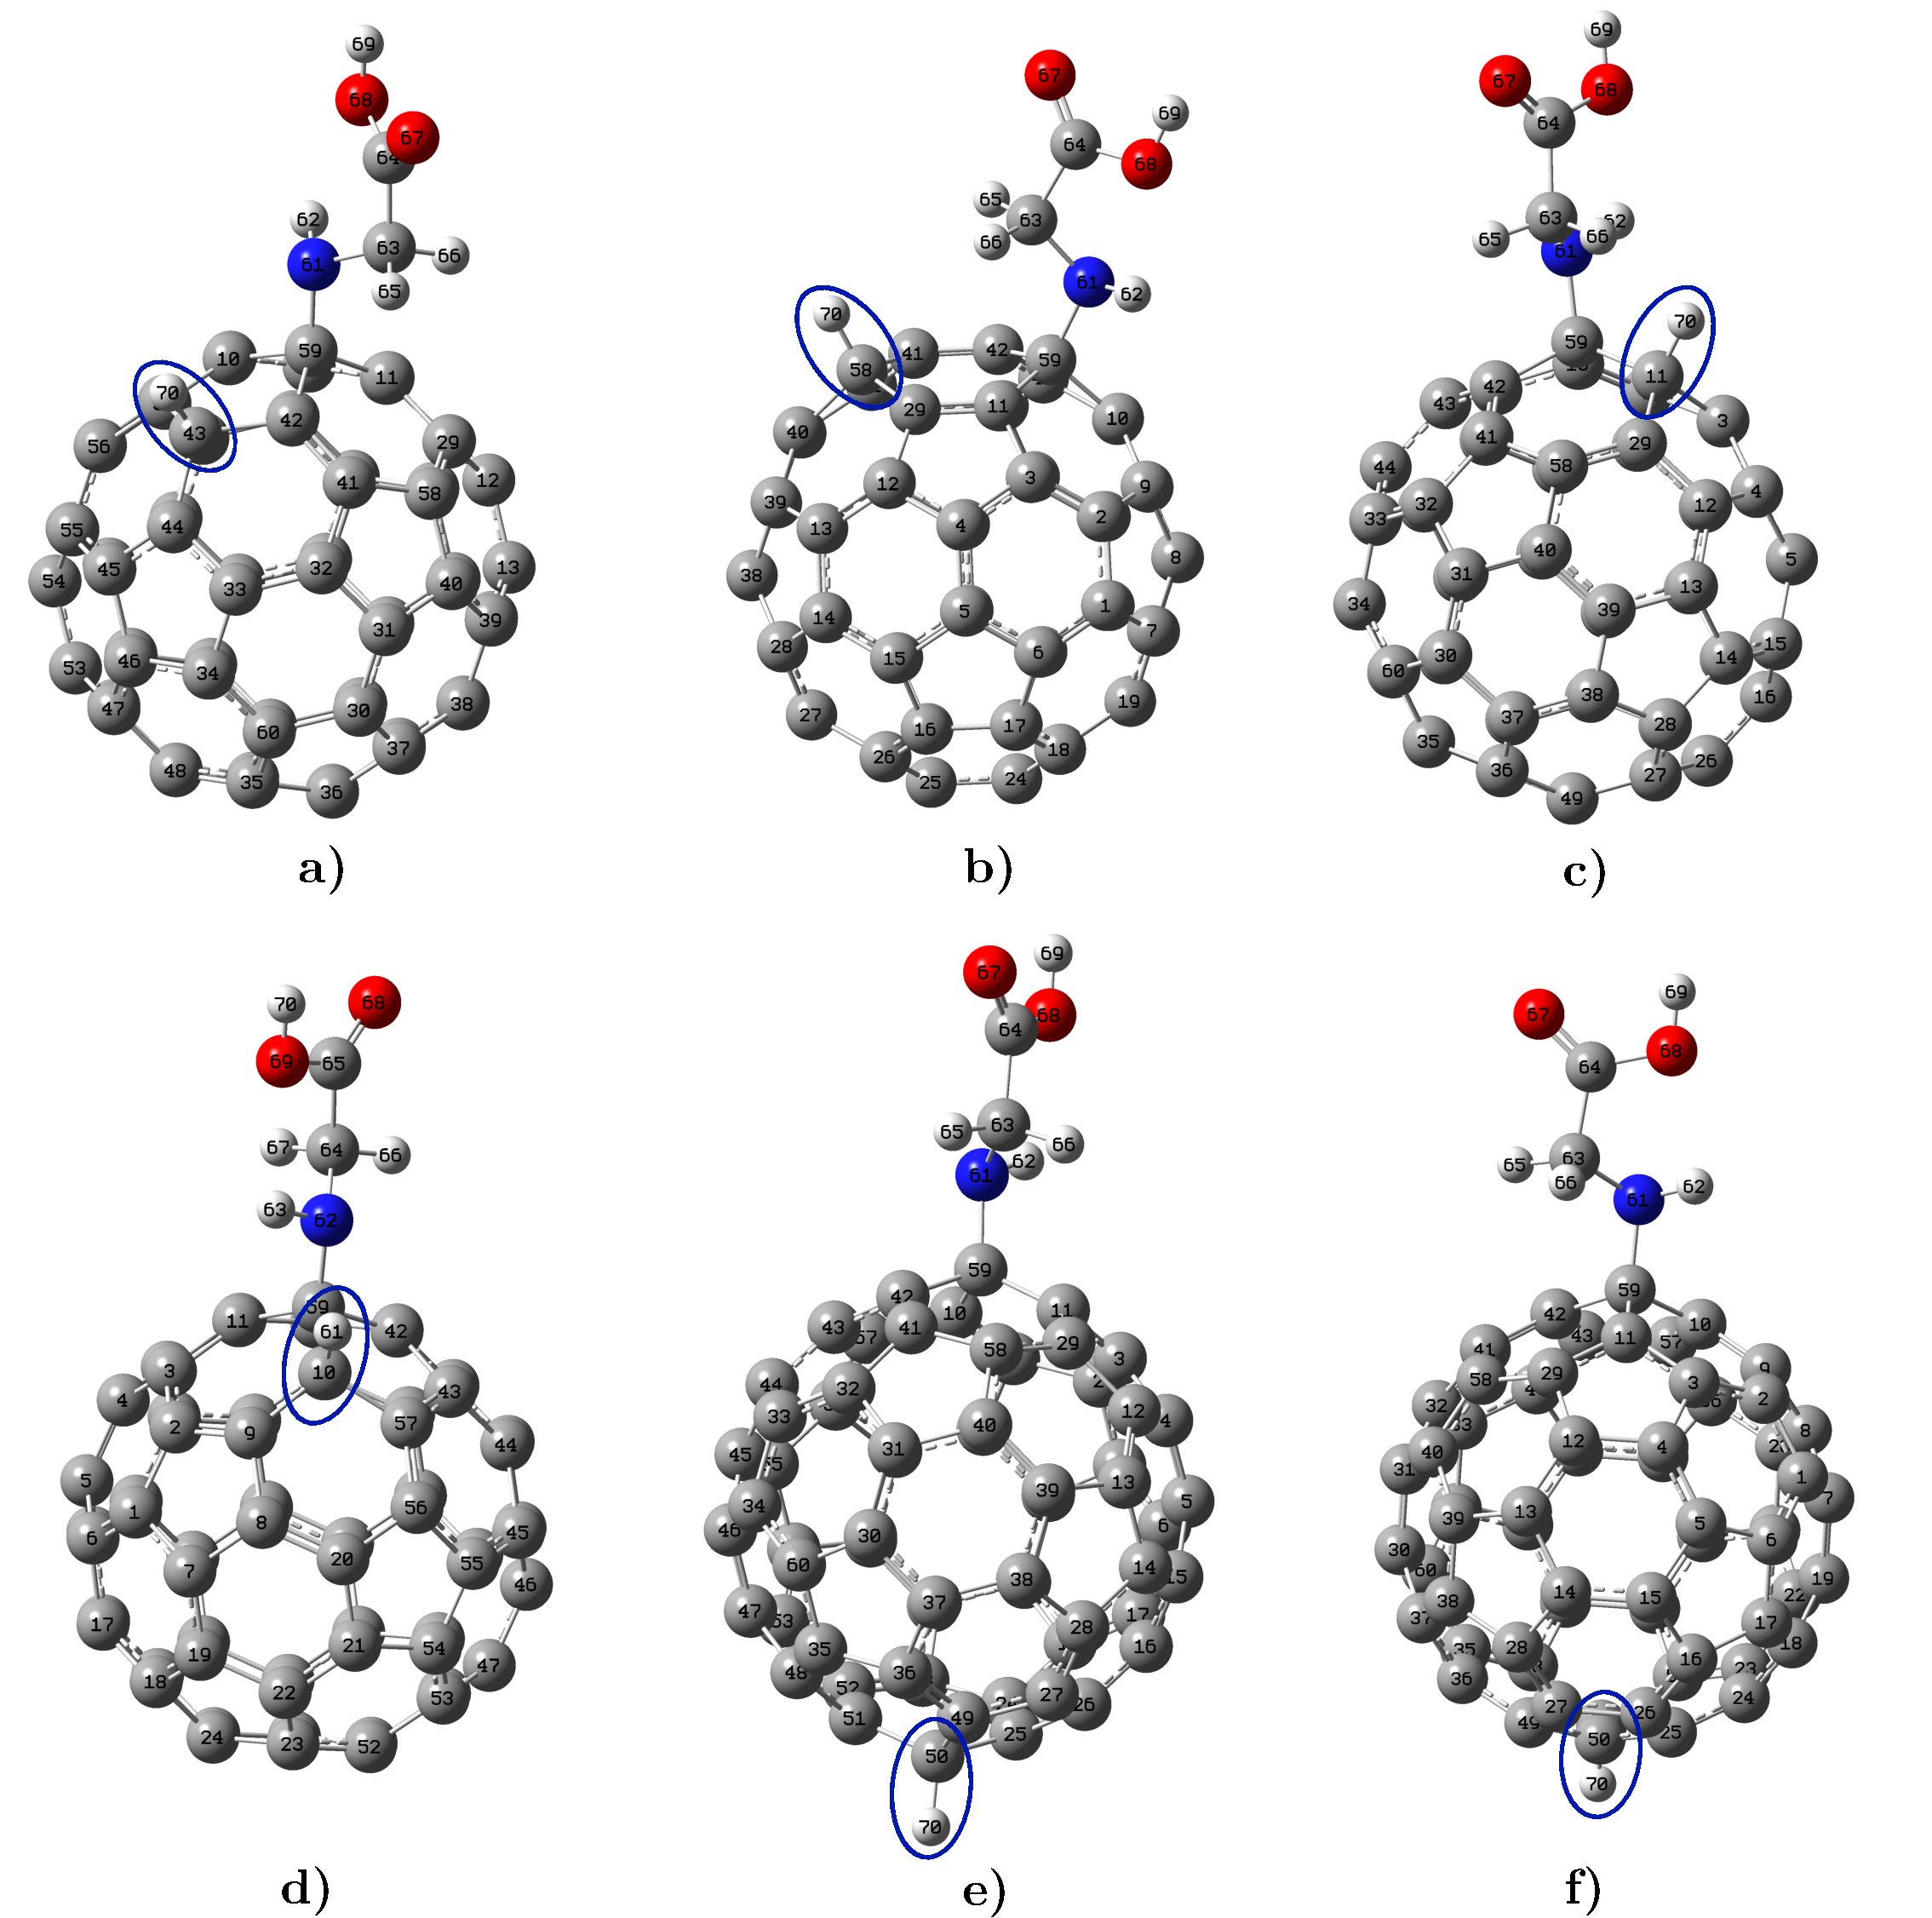
\includegraphics[width=1.0\textwidth]{imagenes/Resu/resu-1-opt.pdf}
      \caption{Isómeros propuestos para la primera adición de glicina al $C_{60}$. La glicina se une al carbono C59; los círculos azules señalan el segundo carbono del enlace evaluado: (a) C43, (b) C58, (c) C11, (d) C10, (e) C50 y (f) C51.}
      \label{fig:isomeros-gly1}
        \end{figure}
        
\begin{figure}[H]
      \centering
      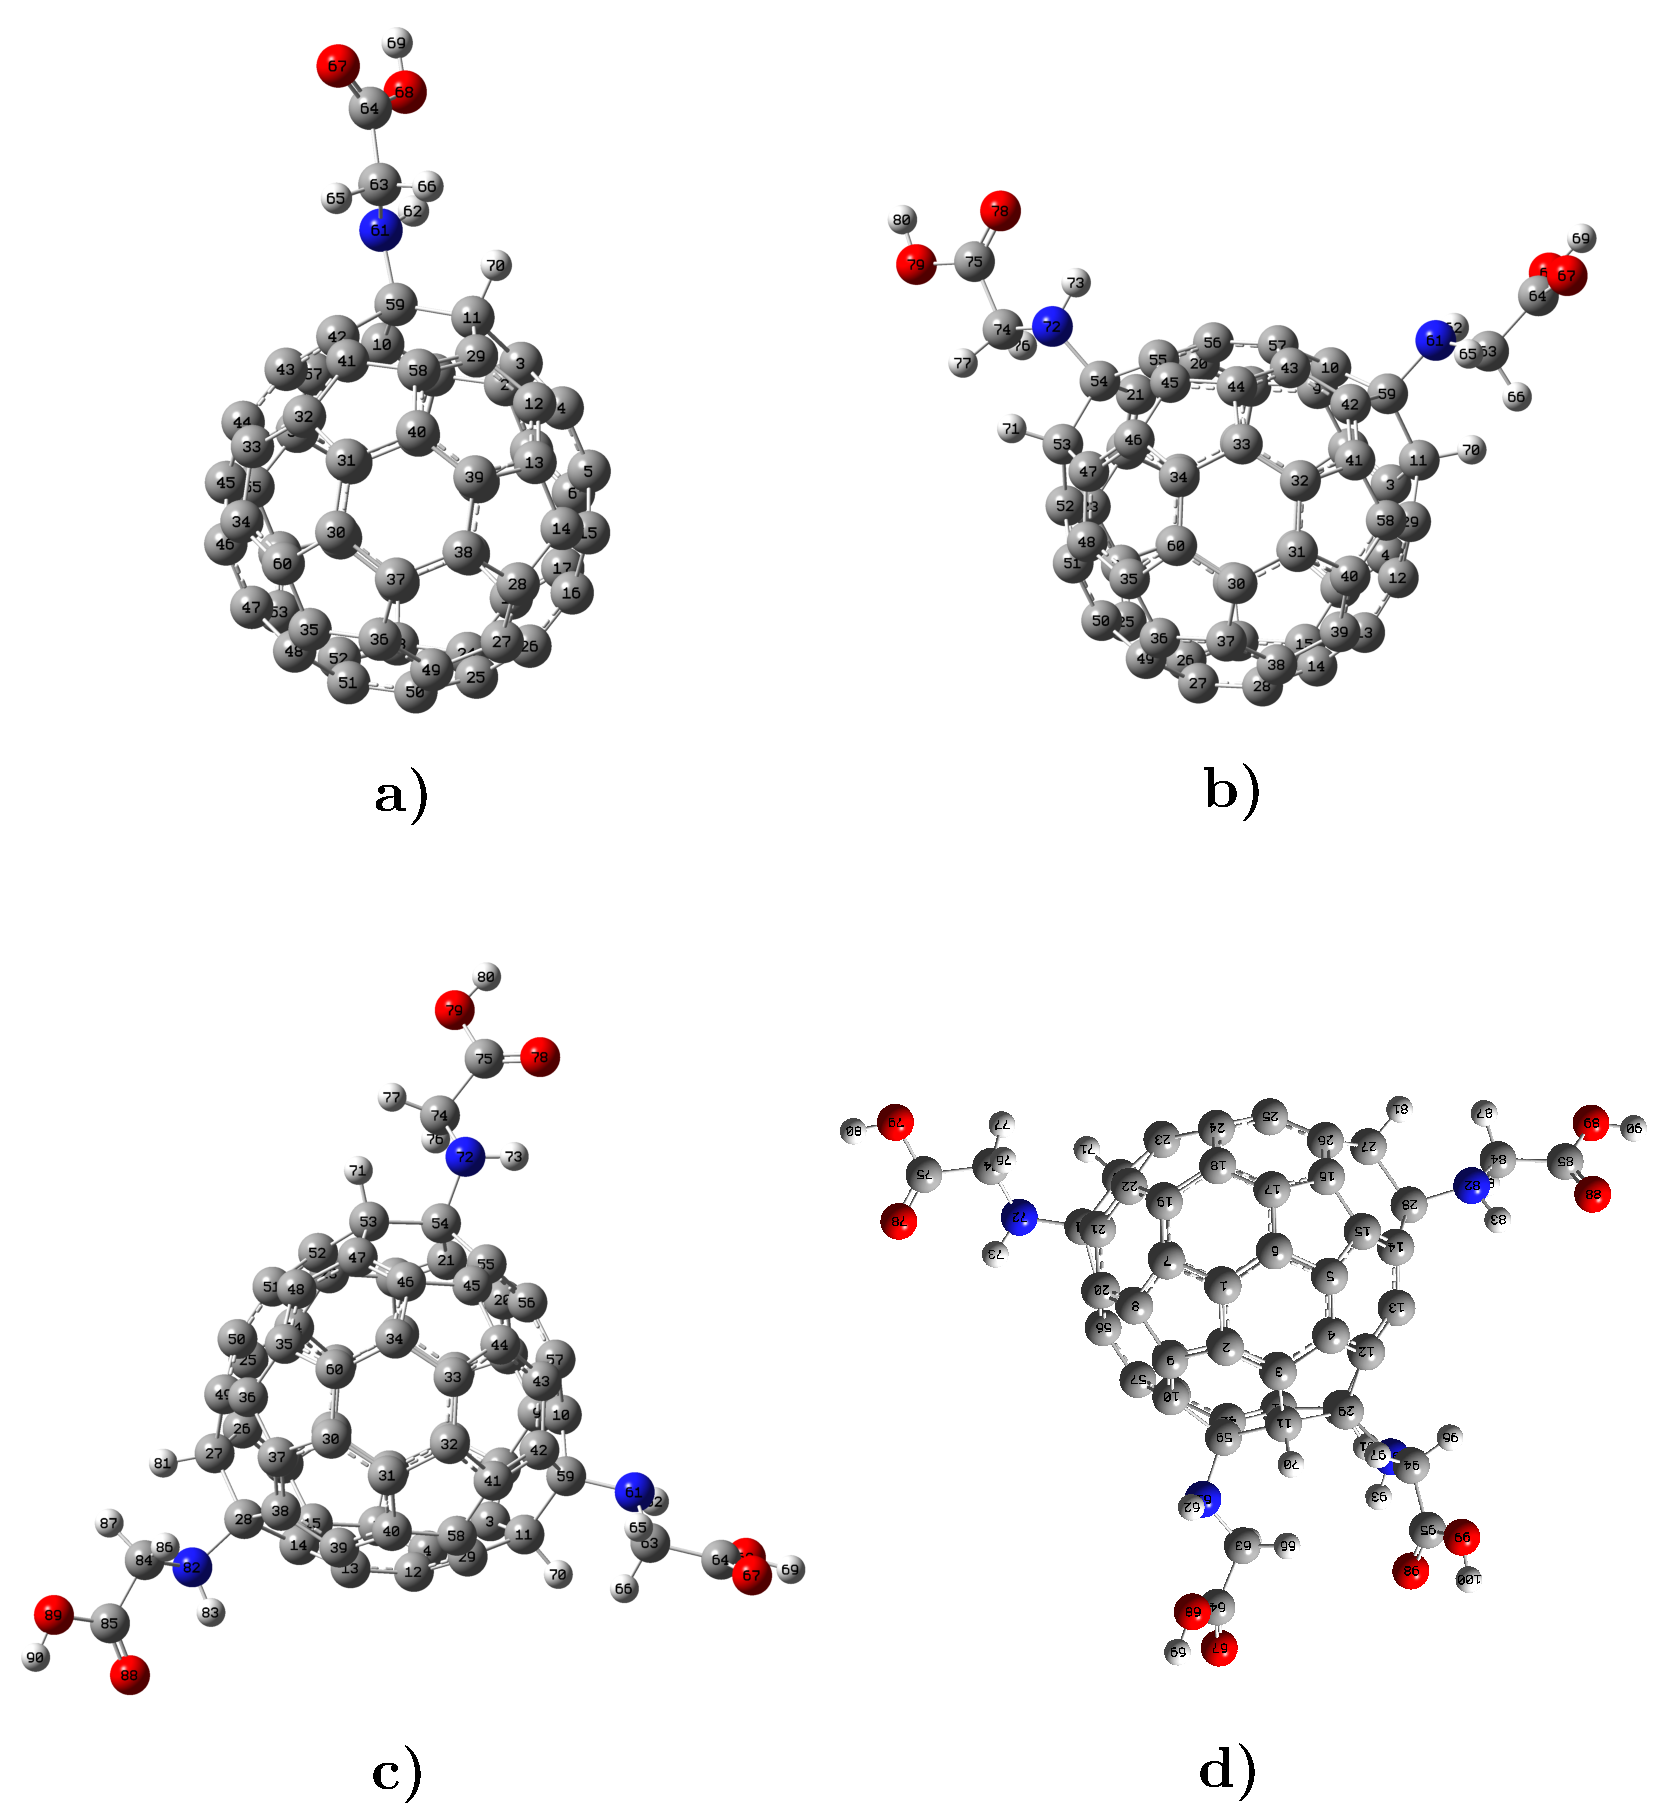
\includegraphics[width=1.0\textwidth]{imagenes/Resu/opt-gly-4.pdf}
      \caption{Estructuras optimizadas de los isómeros evaluados para la segunda adición de glicina al sistema  C\textsubscript{60}(Gly). Los paneles (a)--(d) corresponden a las alternativas estructurales comparadas en esta etapa.}
      \label{fig:isomeros-gly2}
        \end{figure}        

\begin{figure}[H]
      \centering
      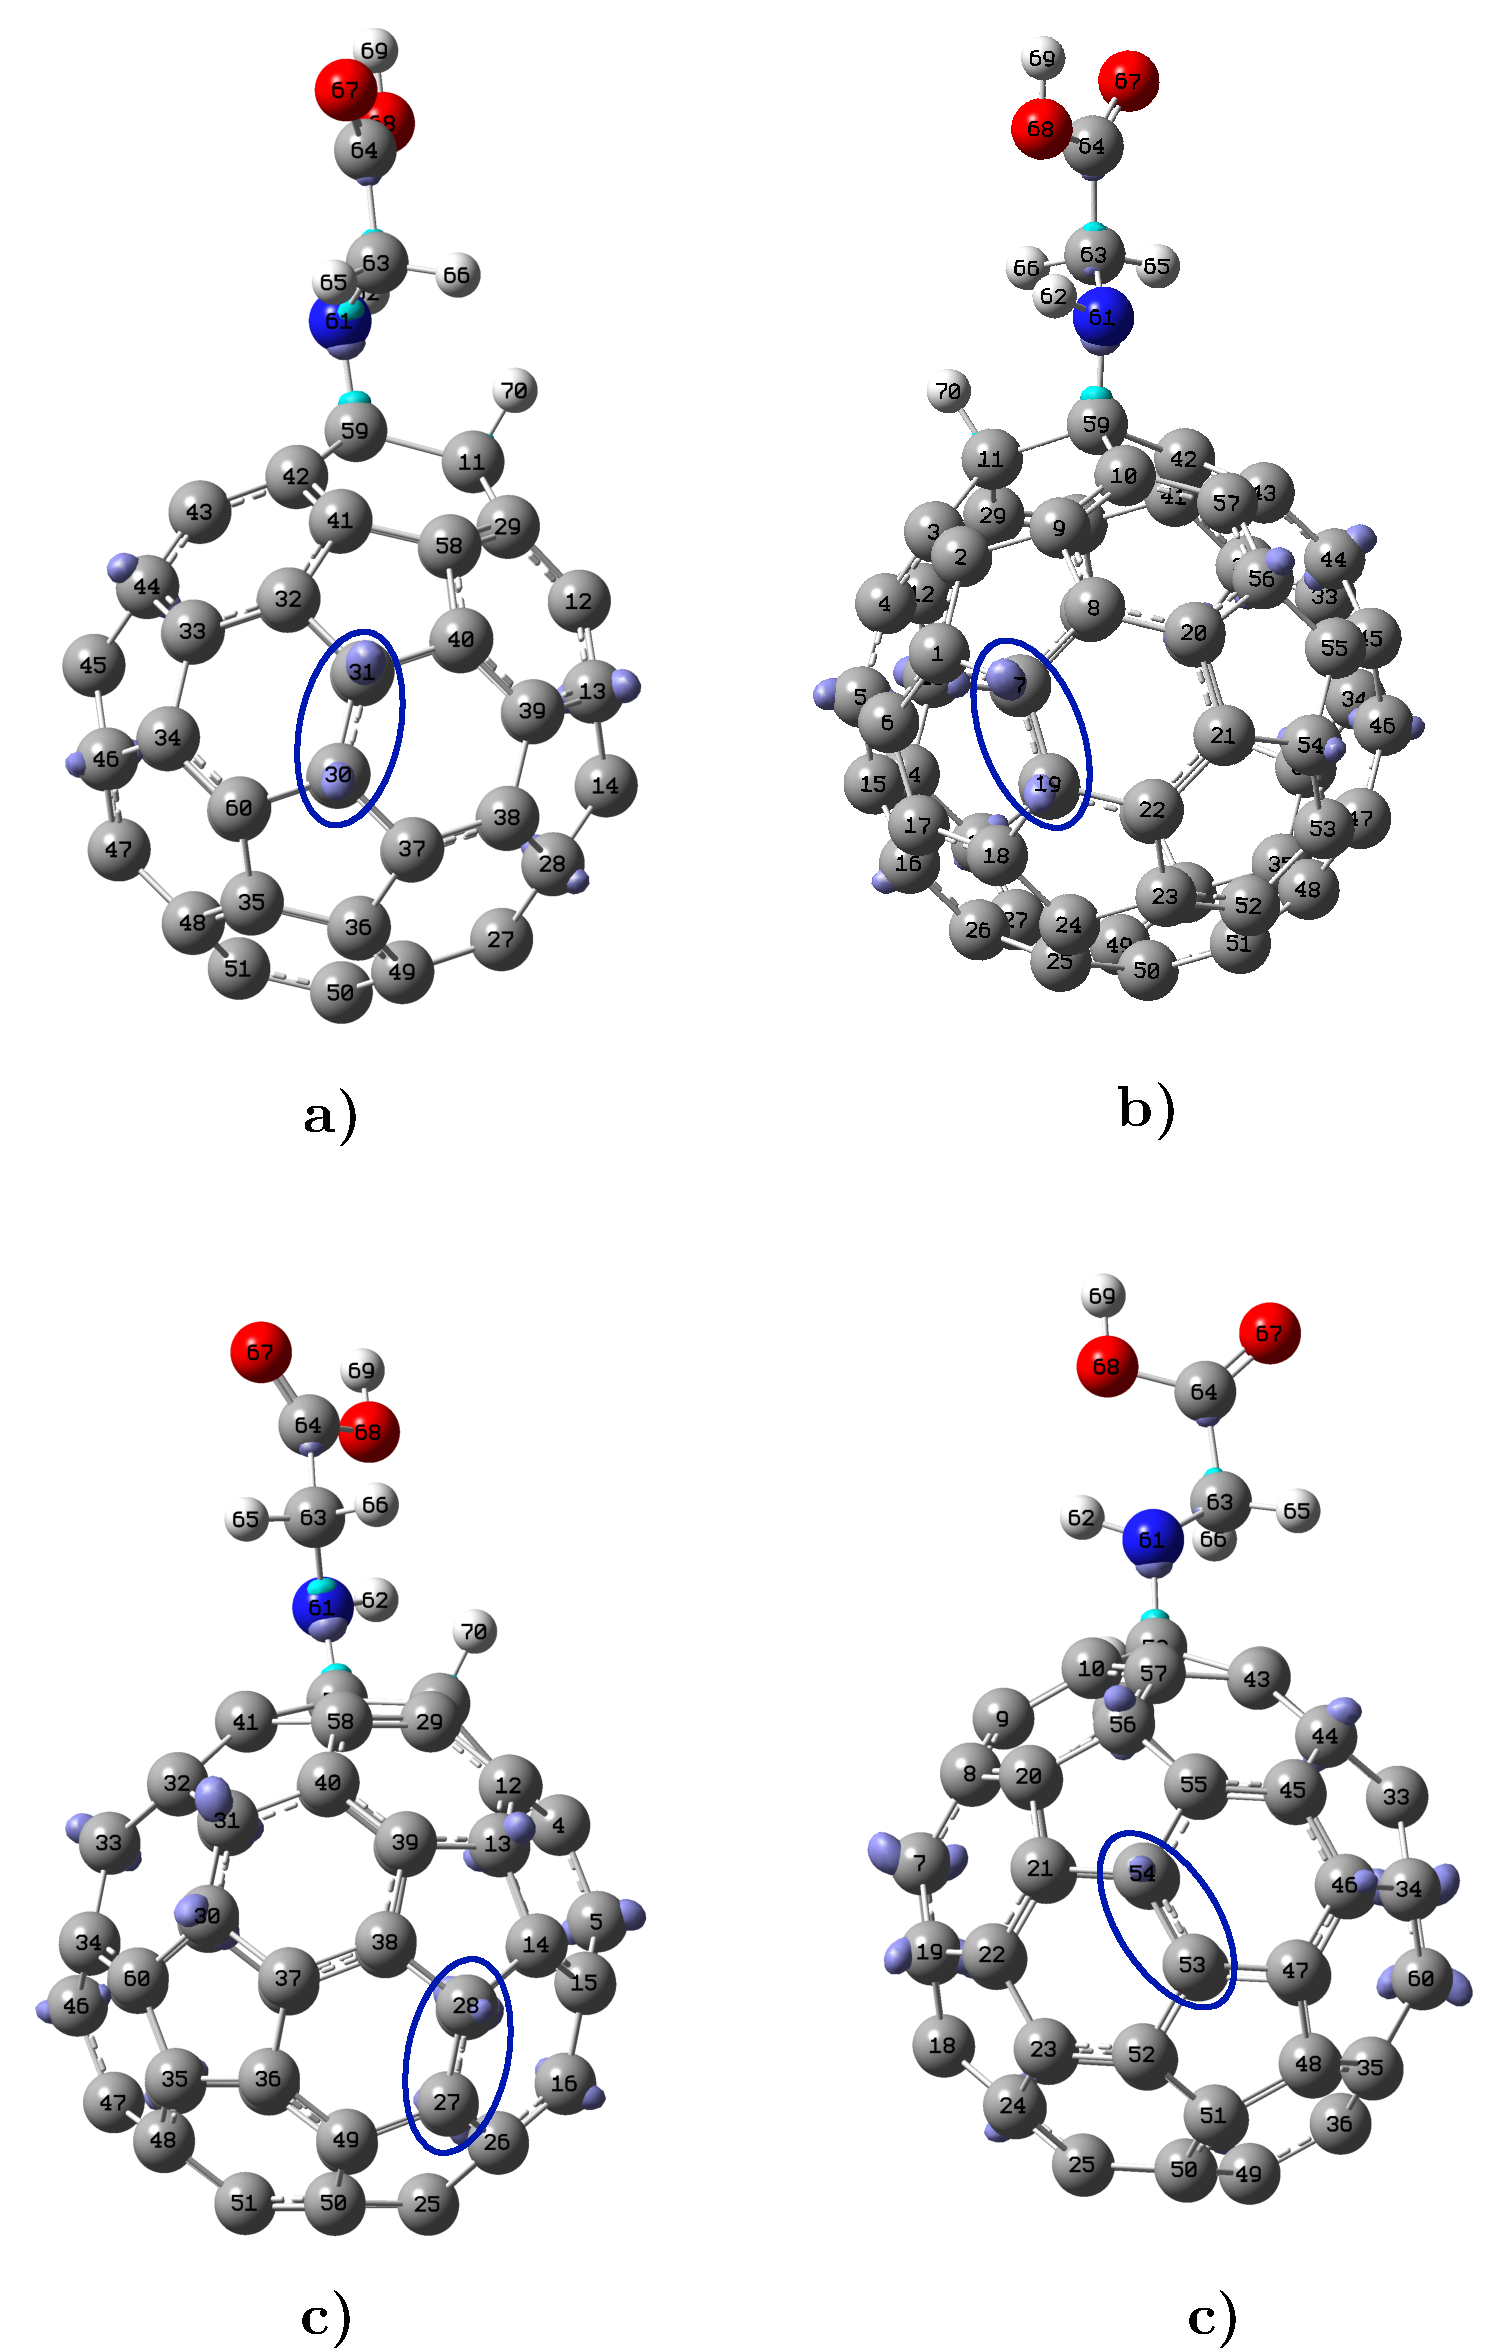
\includegraphics[width=0.7\textwidth]{imagenes/Resu/fukui-gly-resul-1.pdf}
      \caption{Estructuras seleccionadas durante la funcionalización secuencial de la jaula de $C_{60}$ con glicina. Los paneles muestran los sistemas con uno, dos, tres y cuatro grupos de glicina, respectivamente.}
      \label{fig:secuencia-gly}
        \end{figure}

\begin{figure}[H]
      \centering
      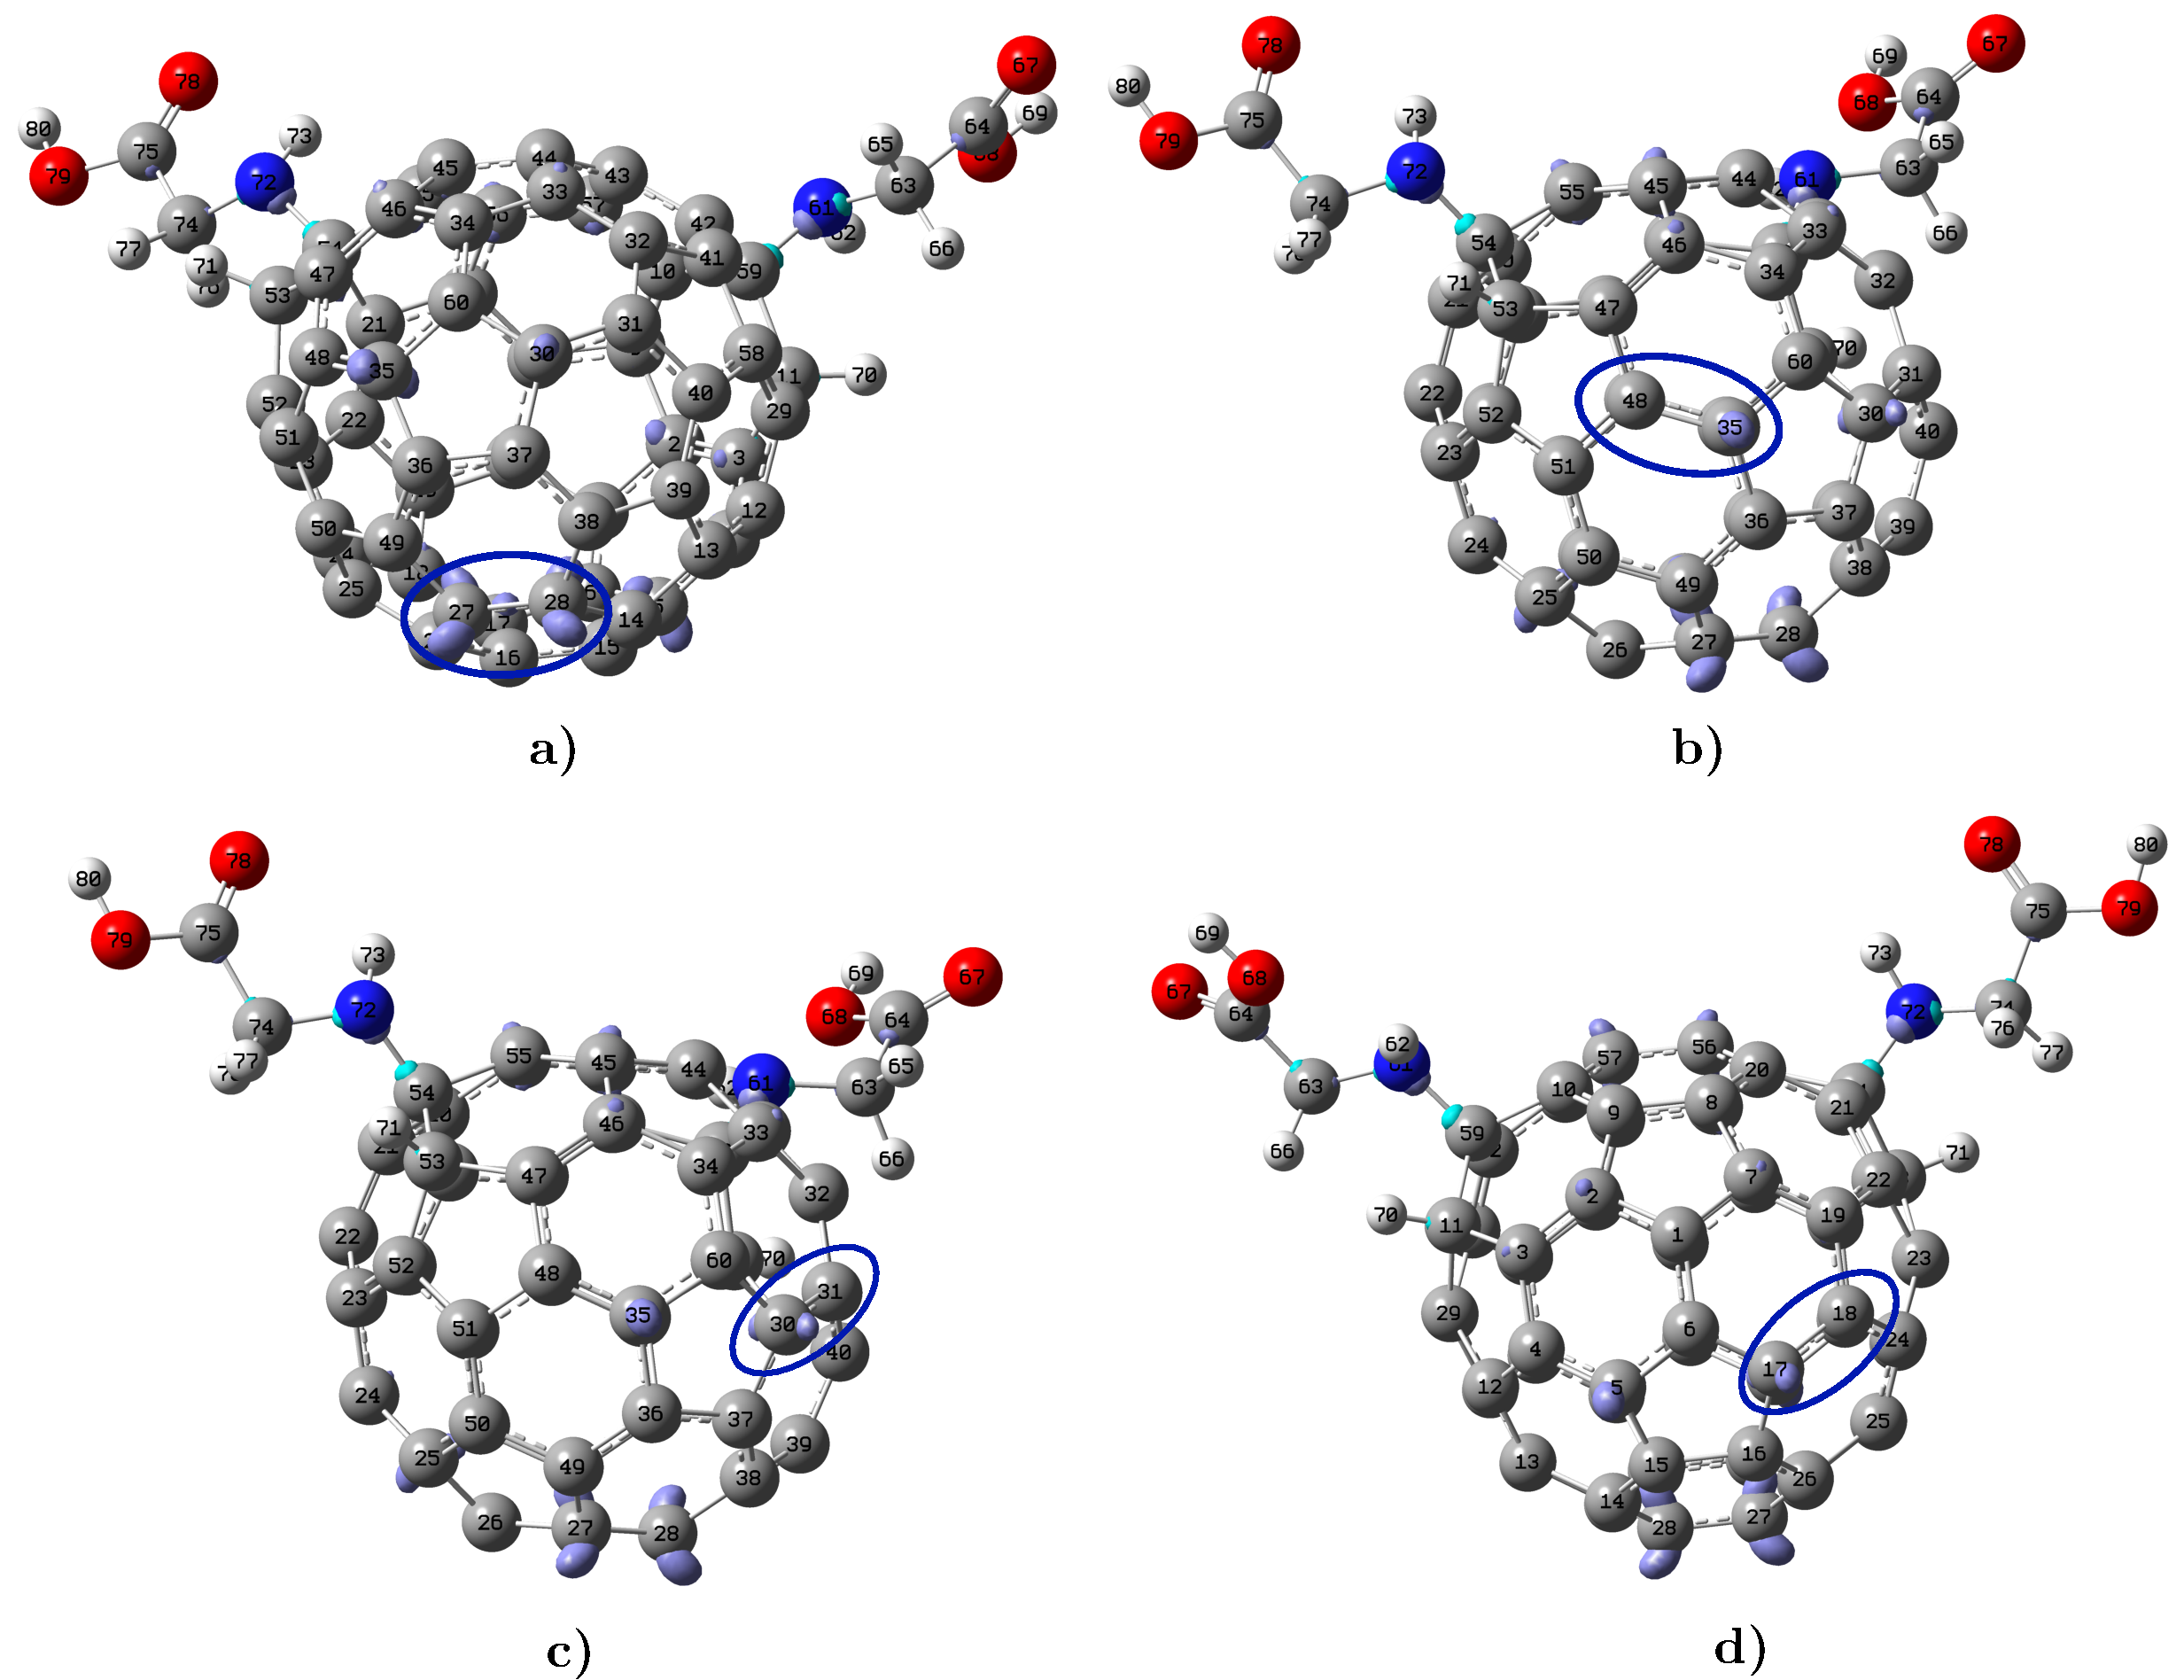
\includegraphics[width=1.0\textwidth]{imagenes/Resu/resu-2-fukui.pdf}
      \caption{Alternativas estructurales consideradas para continuar la funcionalización de $C_{60}$ con un tercer grupo de glicina. Los círculos azules indican los pares de carbonos evaluados como sitios de adición.}
      \label{fig:isomeros-gly3}
        \end{figure}

\begin{figure}[H]
      \centering
      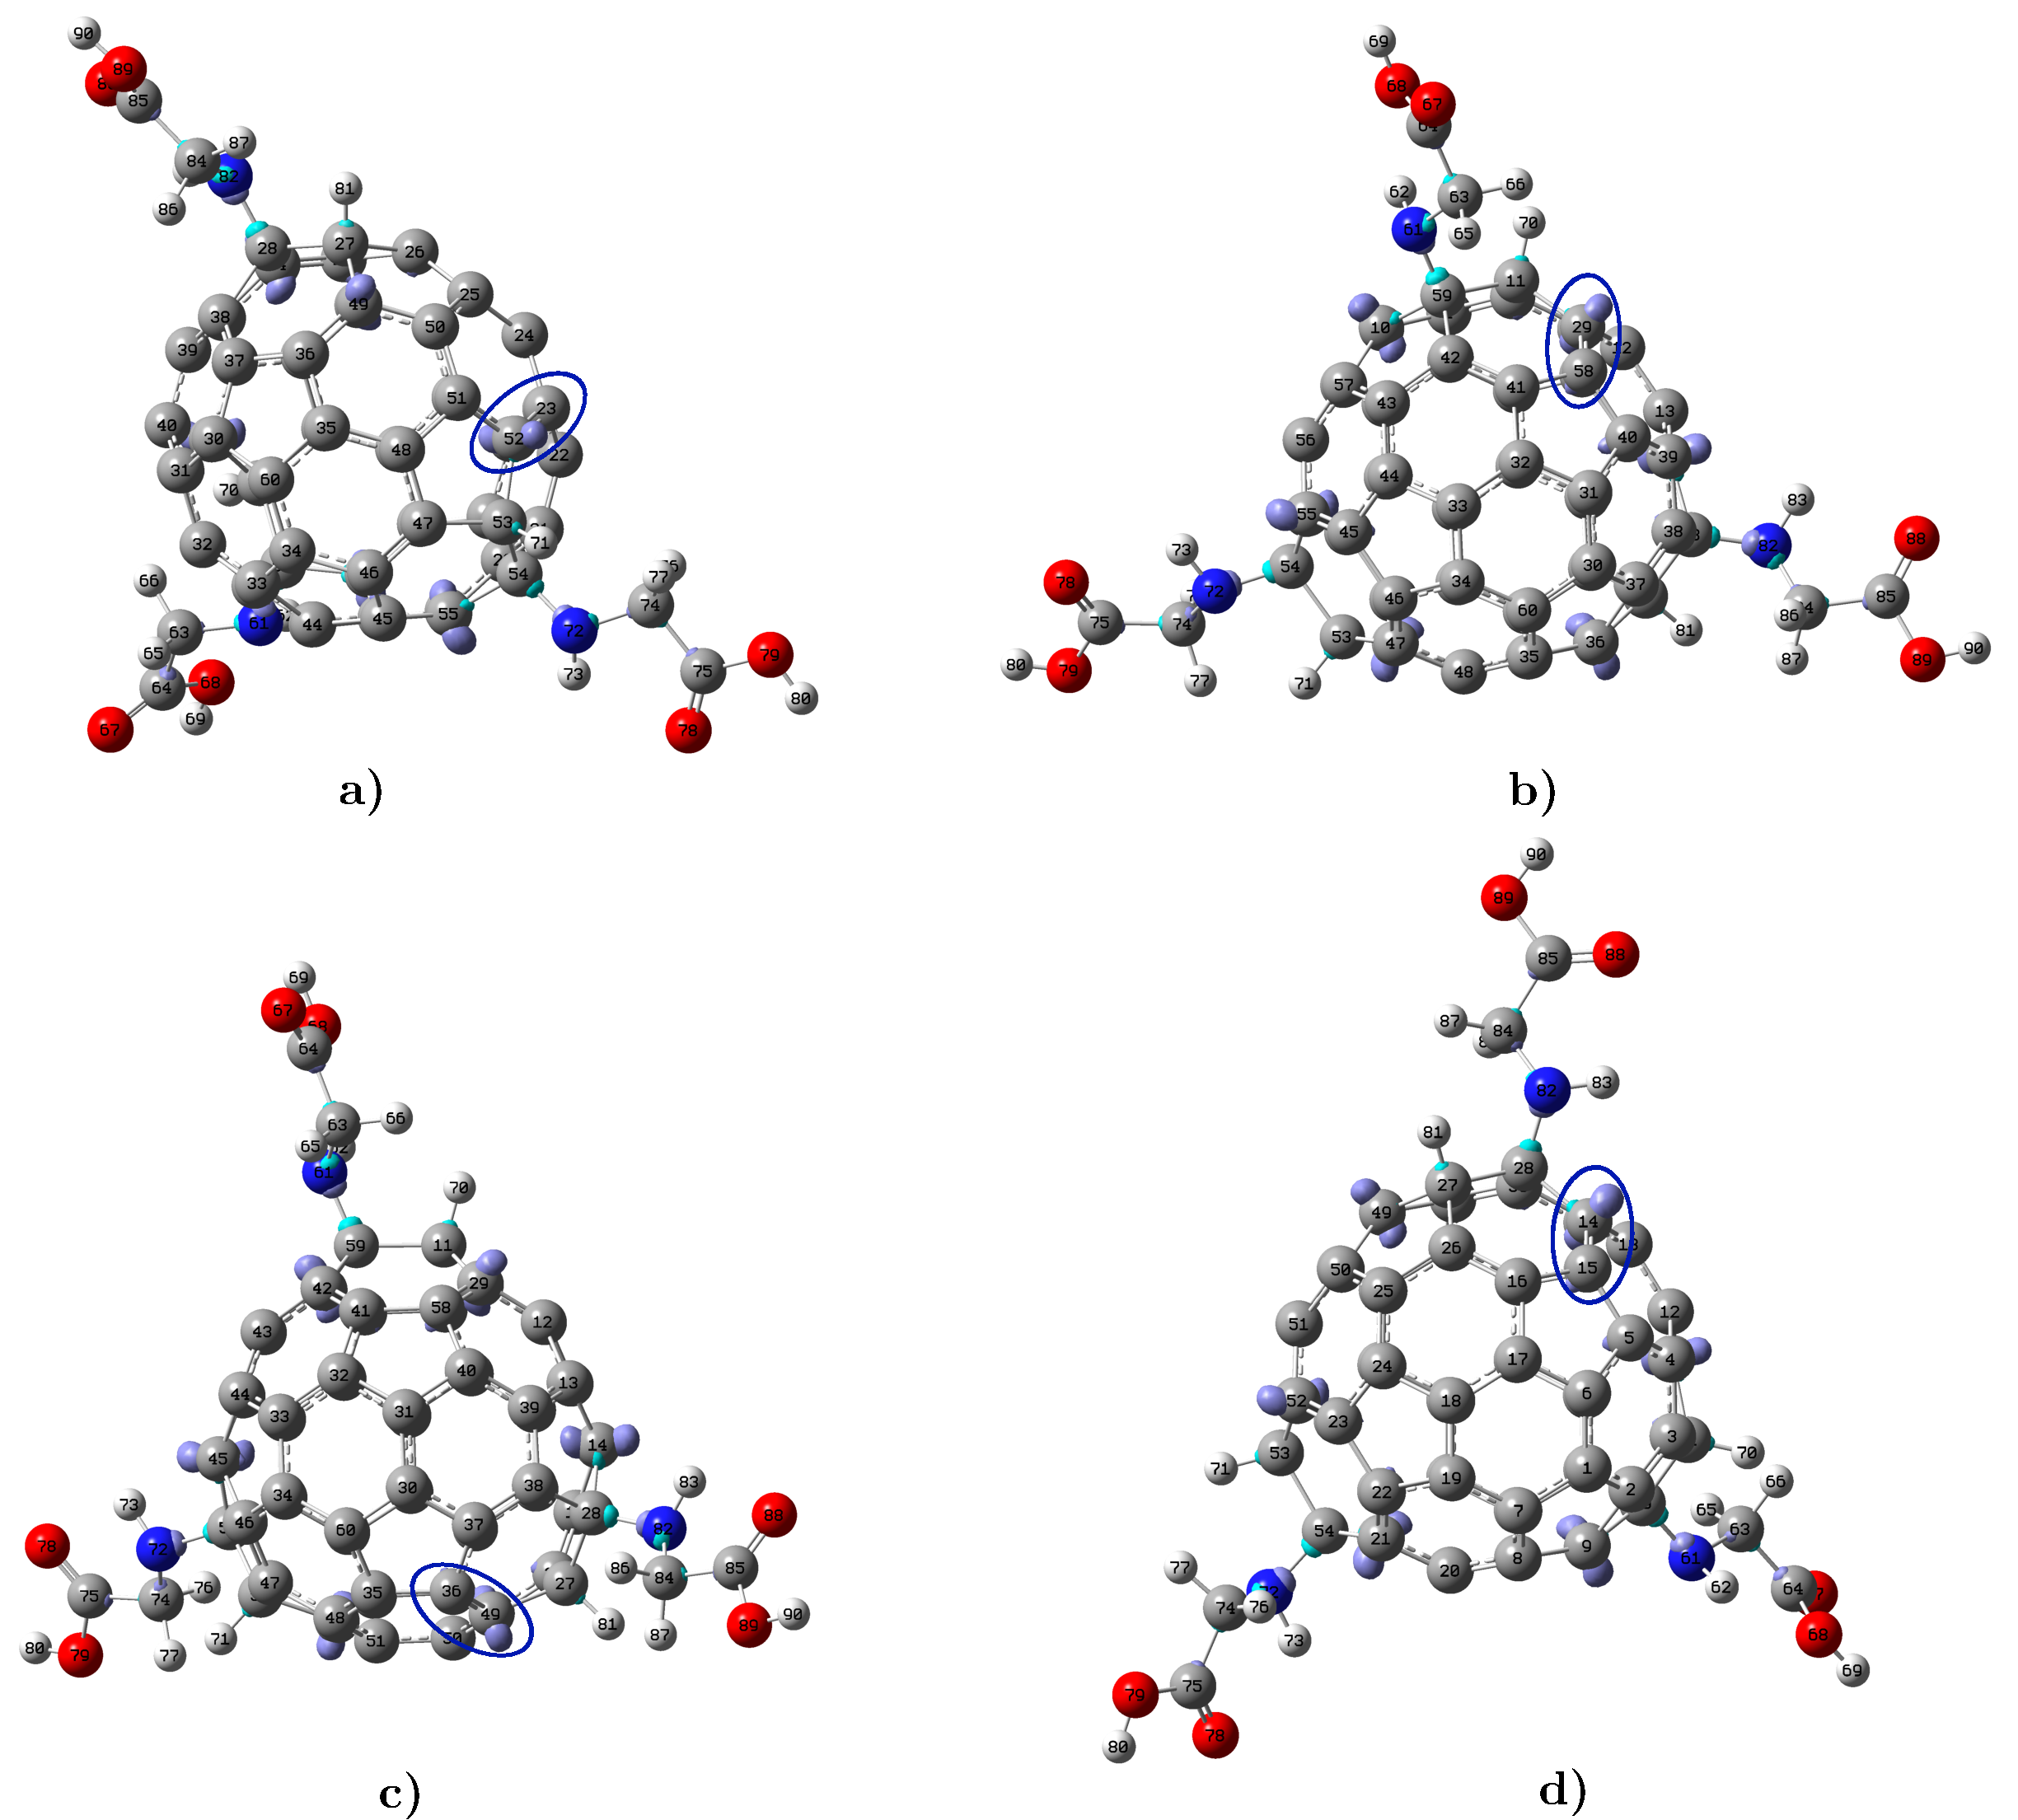
\includegraphics[width=1.0\textwidth]{imagenes/Resu/resu-3-fukui.pdf}
      \caption{Alternativas estructurales consideradas para la cuarta adición de glicina al sistema C\textsubscript{60}(Gly)\textsubscript{3}. Los círculos azules señalan los pares de carbonos analizados para formar el complejo C\textsubscript{60}(Gly)\textsubscript{4}.}
      \label{fig:isomeros-gly4}
        \end{figure}
    
    
 \section{Mecanismo de reacción y cálculo de los índices de reactividad local}

A partir de la optimización del primer aducto $C_{60}(\text{Gly})\text{-c}$, las adiciones sucesivas de las moléculas de glicina se fundamentaron en el análisis de los índices de reactividad local. Dado que la reacción transcurre mediante un mecanismo de adición nucleofílica donde el grupo amino de la glicina actúa como especie nucleófila y la jaula de $C_{60}$ como electrófilo, se calcularon las \textbf{funciones de Fukui para ataque nucleofílico ($f^+$)} sobre la superficie del sistema en cada etapa de funcionalización.

Las regiones de la jaula con mayor susceptibilidad reactiva se identificaron mediante la visualización de los lóbulos de densidad electrónica en las funciones de Fukui empleando un isovalor de $0.003\text{ a.u.}$ (Figuras~\ref{fig:secuencia-gly}, \ref{fig:secuencia-gly2}, \ref{fig:isomeros-gly3}) y \ref{fig:isomeros-gly4}). Los sitios de mayor reactividad se concentraron predominantemente sobre enlaces de tipo [6,6], los cuales conservan un mayor carácter de doble enlace y menor tensión de anillo. Las propuestas para las adiciones 2, 3 y 4 se establecieron estrictamente sobre las zonas donde los lóbulos mostraron las mayores magnitudes de reactividad local.

\section{Análisis de las adiciones secuenciales ($C_{60}(\text{Gly})_2$ a $C_{60}(\text{Gly})_4$)}

\paragraph{Segunda adición: $C_{60}(\text{Gly})_2$}
Para la formación del complejo difuncionalizado se evaluaron cuatro sitios candidatos propuestos a partir de los mapas de Fukui (Tabla~\ref{tab:adicion-secuencial-gly}). Como se observa en los resultados energéticos, la \textbf{Propuesta 4} (carbonos C54, C53) presentó la mayor estabilidad termodinámica, definíendose como la estructura de referencia ($0.000\text{ kcal mol}^{-1}$). Aunque las diferencias respecto a las demás alternativas no superan las $0.850\text{ kcal mol}^{-1}$ (candidatos 1, 2 y 3 con $0.696$, $0.789$ y $0.850\text{ kcal mol}^{-1}$, respectivamente), la ligera preferencia energética hacia la posición C54--C53 se atribuye a una menor repulsión estérica entre las cadenas de glicina y a una distribución electrónica de la red optimizada tras el primer ataque.

\paragraph{Tercera adición: $C_{60}(\text{Gly})_3$}
En la evaluación de la tercera molécula de glicina (Figura~\ref{fig:isomeros-gly3}), el mapa de reactividad de Fukui sobre $C_{60}(\text{Gly})_2$ identificó cuatro nuevas regiones objetivo. Entre ellas, la \textbf{Propuesta 1} (carbonos C28, C27) resultó ser el mínimo global con $0.000\text{ kcal mol}^{-1}$. A diferencia de la etapa anterior, en esta adición se observa una clara diferenciación energética: la Propuesta 2 (C35, C48) se encuentra fuertemente desestabilizada a $+3.935\text{ kcal mol}^{-1}$, mientras que las Propuestas 3 (C30, C31) y 4 (C17, C18) se ubican a $+1.142$ y $+1.208\text{ kcal mol}^{-1}$, respectivamente. Este incremento en la barrera termodinámica evidencia que la acumulación de tres grupos voluminosos sobre la jaula comienza a generar un impedimento estérico significativo y una pertubación considerable sobre la conjugación $\pi$ cíclica.

\paragraph{Cuarta adición: $C_{60}(\text{Gly})_4$}
Finalmente, para la tetrafuncionalización (Figura~\ref{fig:isomeros-gly4}), el análisis de reactividad sobre $C_{60}(\text{Gly})_3$ permitió formular cuatro propuestas finales. La \textbf{Propuesta 2} (carbonos C29, C58) mostró la mayor estabilidad termodinámica ($0.000\text{ kcal mol}^{-1}$), seguida de cerca por la Propuesta 3 (C49, C36 a $+0.640\text{ kcal mol}^{-1}$) y la Propuesta 1 (C52, C23 a $+0.676\text{ kcal mol}^{-1}$), mientras que la Propuesta 4 (C14, C15) resultó ser la menos favorable ($+2.180\text{ kcal mol}^{-1}$). 

La estrecha cercanía energética entre las tres primeras propuestas ($< 0.7\text{ kcal mol}^{-1}$) ocurre debido a que corresponden a enlaces [6,6] topológicamente equivalentes dentro de los dominios no funcionalizados de la jaula. Sin embargo, la ventaja energética sutil de la Propuesta 2 (C29, C58) está dictada por las interacciones intramoleculares secundarias, tales como el posible ordenamiento de los protones libres. Estas interacciones modulan la reactividad local de Fukui y determinan la configuración de mayor estabilidad para el sistema final $C_{60}(\text{Gly})_4$ Figura~\ref{fig:isomeros-gly4}.  
\section{Análisis de descriptores de reactividad global PI y AE)}
\begin{table}[H]
    \centering
    \caption{Energías totales calculadas en kcal/mol para la glicina, el fullereno $C_{60}$ y el sistema funcionalizado  C\textsubscript{60}(Gly).}
    \label{tab:energias-referencia}
    \renewcommand{\arraystretch}{1.15}
    \begin{tabular}{lccc}
        \toprule
        \textbf{Sistema} & \textbf{PI (eV)} & \textbf{AE (eV)}\\
        \midrule
         C\textsubscript{60}(Gly)\textsubscript{4} & 6.849
 & 1.779 \\
        Fullereno  C\textsubscript{60} & 7.608
 & 2.454 \\
        \bottomrule
    \end{tabular}
\end{table}
{Análisis de parámetros de reactividad global y potencial biológico}

El análisis de los parámetros reactivos globales presentados en la Tabla~\ref{tab:energias-referencia} revela modificaciones sustanciales en las propiedades electrónicas del fulereno tras la tetrafuncionalización con glicina. Se observa una reducción significativa en el Potencial de Ionización ($PI$), pasando de $7.608\text{ eV}$ en el $C_{60}$ prístino a $6.849\text{ eV}$ en el complejo $C_{60}(\text{Gly})_4$. Un valor menor de $PI$ indica que la energía del orbital molecular ocupado de mayor energía (HOMO) se ha elevado, disminuyendo la barrera energética requerida para la extracción de un electrón. Esta mayor facilidad para la donación electrónica posiciona al sistema $C_{60}(\text{Gly})_4$ como un potente agente reductor y antioxidante, capaz de neutralizar Especies Reactivas de Oxígeno (ROS) en entornos celulares mediante mecanismos de transferencia de un electrón (SET).

Por otro lado, la Afinidad Electrónica ($AE$) experimentó una disminución desde $2.454\text{ eV}$ en la jaula prístina hasta $1.779\text{ eV}$ en el aducto $C_{60}(\text{Gly})_4$. Mientras que el $C_{60}$ sin funcionalizar actúa primordialmente como un aceptor de electrones altamente eficiente debido a su elevada $AE$, la adición de los cuatro residuos de glicina modula el carácter amfotérico de la jaula, atenuando la capacidad electroatractora e incrementando fuertemente el perfil electrodonador.

En conjunto, la funcionalización secuencial con glicina cumple un doble propósito de alto valor biomédico: por un lado, incrementa la capacidad antioxidante del sistema al reducir el $PI$; por otro, introduce grupos funcionales polares ($-\text{COOH}$ y $-\text{NH}_2$) que le confieren solubilidad en medios acuosos y biocompatibilidad, superando la principal limitación de insolubilidad del $C_{60}$ prístino en medios fisiológicos.


    
    \section{Potencial electrostático superficial}
     \begin{table}[H]
    \centering
    \caption{Valores de potencial electrostático para cada sistema de C\textsubscript{60}(Gly).}
    \label{tab:potencial-electrostatico}
    \renewcommand{\arraystretch}{1.15}
    \begin{tabular}{lc}
        \toprule
        \textbf{Sistema} & \textbf{Valor de potencial electrostático} \\
        \midrule
        Fullereno C\textsubscript{60}(Gly) & 1.465 \\
       C\textsubscript{60}(Gly) & 0.975 \\
        C\textsubscript{60}(Gly)\textsubscript{2} & 2.289 \\
        C\textsubscript{60}(Gly)\textsubscript{3} & 2.556 \\
        C\textsubscript{60}(Gly)\textsubscript{4} & 6.024 \\
        \midrule
        \textbf{Promedio} & \textbf{2.662} \\
        \bottomrule
        \end{tabular}
\end{table}

El análisis del Potencial Electrostático Superficial (MEP) presentado en la Tabla~\ref{tab:potencial-electrostatico} revela una clara tendencia hacia la electropositividad a medida que avanza la funcionalización secuencial del $C_{60}$. En el aducto monofuncionalizado $C_{60}(\text{Gly})$, el potencial promedio se sitúa en $0.975\text{ kcal mol}^{-1}$; sin embargo, la incorporación progresiva de residuos de aminoácido provoca un incremento sustancial hasta alcanzar un valor máximo de $6.024\text{ kcal mol}^{-1}$ en el complejo tetrafuncionalizado $C_{60}(\text{Gly})_4$. 

Este marcado desplazamiento hacia un perfil predominantemente electropositivo en el $C_{60}(\text{Gly})_4$ —el cual supera en más de cuatro veces al valor del $C_{60}$ prístino ($1.466\text{ kcal mol}^{-1}$)— se explica por la acumulación neta de protones ($H$) pertenecientes a los grupos $-\text{NH}_2$ y $-\text{COOH}$. Como se observa en el análisis atómico de la Figura~\ref{fig:esp-promedio}, la densidad electropositiva individual de los protones (con picos que superan los $+30\text{ kcal mol}^{-1}$) termina por dominar el promedio global del sistema sobre los aportes electronegativos de los átomos de oxígeno y nitrógeno (localizados en torno a $-20\text{ kcal mol}^{-1}$).

\subsection{Implicaciones en el reconocimiento molecular con la proteína 2FOM (DENV2)}

Desde la perspectiva del reconocimiento molecular, el elevado carácter electropositivo global alcanzado en el sistema $C_{60}(\text{Gly})_4$ constituye un factor determinante para sus aplicaciones biológicas. Específicamente, en la proteína de envoltura del virus del Dengue serotipo 2 (DENV2, PDB ID: 2FOM), la arquitectura del sitio activo y de diversas cavidades de superficie cuenta con una alta densidad de aminoácidos aniónicos (tales como ácido aspártico y ácido glutámico), los cuales generan campos de potencial electrostático fuertemente negativos.

Por consiguiente, el incremento en la electropositividad del derivado tetrafuncionalizado actúa como un potente impulsor termodinámico, favoreciendo una atracción electrostática de largo alcance hacia estas cavidades aniónicas de la proteína 2FOM. Al mismo tiempo, la presencia de polos electronegativos locales en los oxígenos/nitrógenos y las regiones neutras sobre la jaula de $C_{60}$ (visibles en el mapa tridimensional de la Figura~\ref{fig:mep-gly4}) le otorgan al ligando la versatilidad necesaria para establecer puentes de hidrógeno secundarios y contactos hidrofóbicos, garantizando un acoplamiento molecular estable y específico en el dominio biológico evaluado.


Los valores de la Tabla~\ref{tab:potencial-electrostatico} muestran que la funcionalización con glicina modifica el potencial electrostático promedio del sistema. El fullereno presenta un valor de 1.466, mientras que la primera adición de glicina reduce este valor a 0.975. A partir de la segunda adición, el potencial aumenta a 2.289 y 2.556 para los sistemas con dos y tres glicinas, respectivamente, hasta alcanzar 6.024 en C\textsubscript{60}(Gly)\textsubscript{4}. Por lo tanto, el cambio no es lineal en la primera etapa, pero la tendencia general a partir de la segunda incorporación indica que los grupos de glicina afectan de manera importante la distribución electrónica de la superficie molecular.

La Figura~\ref{fig:esp-promedio} permite observar esta variación a nivel de los sitios evaluados. La coexistencia de valores positivos y negativos indica que la superficie del sistema no es uniforme y que conserva regiones con distinto carácter electrostático. Conforme aumenta el número de grupos de glicina, estas regiones se redistribuyen alrededor de la jaula de C\textsubscript{60}(Gly), lo cual es consistente con la incorporación de grupos funcionales polares. El mapa de potencial electrostático de la Figura~\ref{fig:mep-gly4} complementa este resultado al mostrar que, en el sistema con cuatro glicinas, las zonas de mayor variación se localizan principalmente alrededor de los sustituyentes.
    
    \begin{figure}[H]
      \centering
      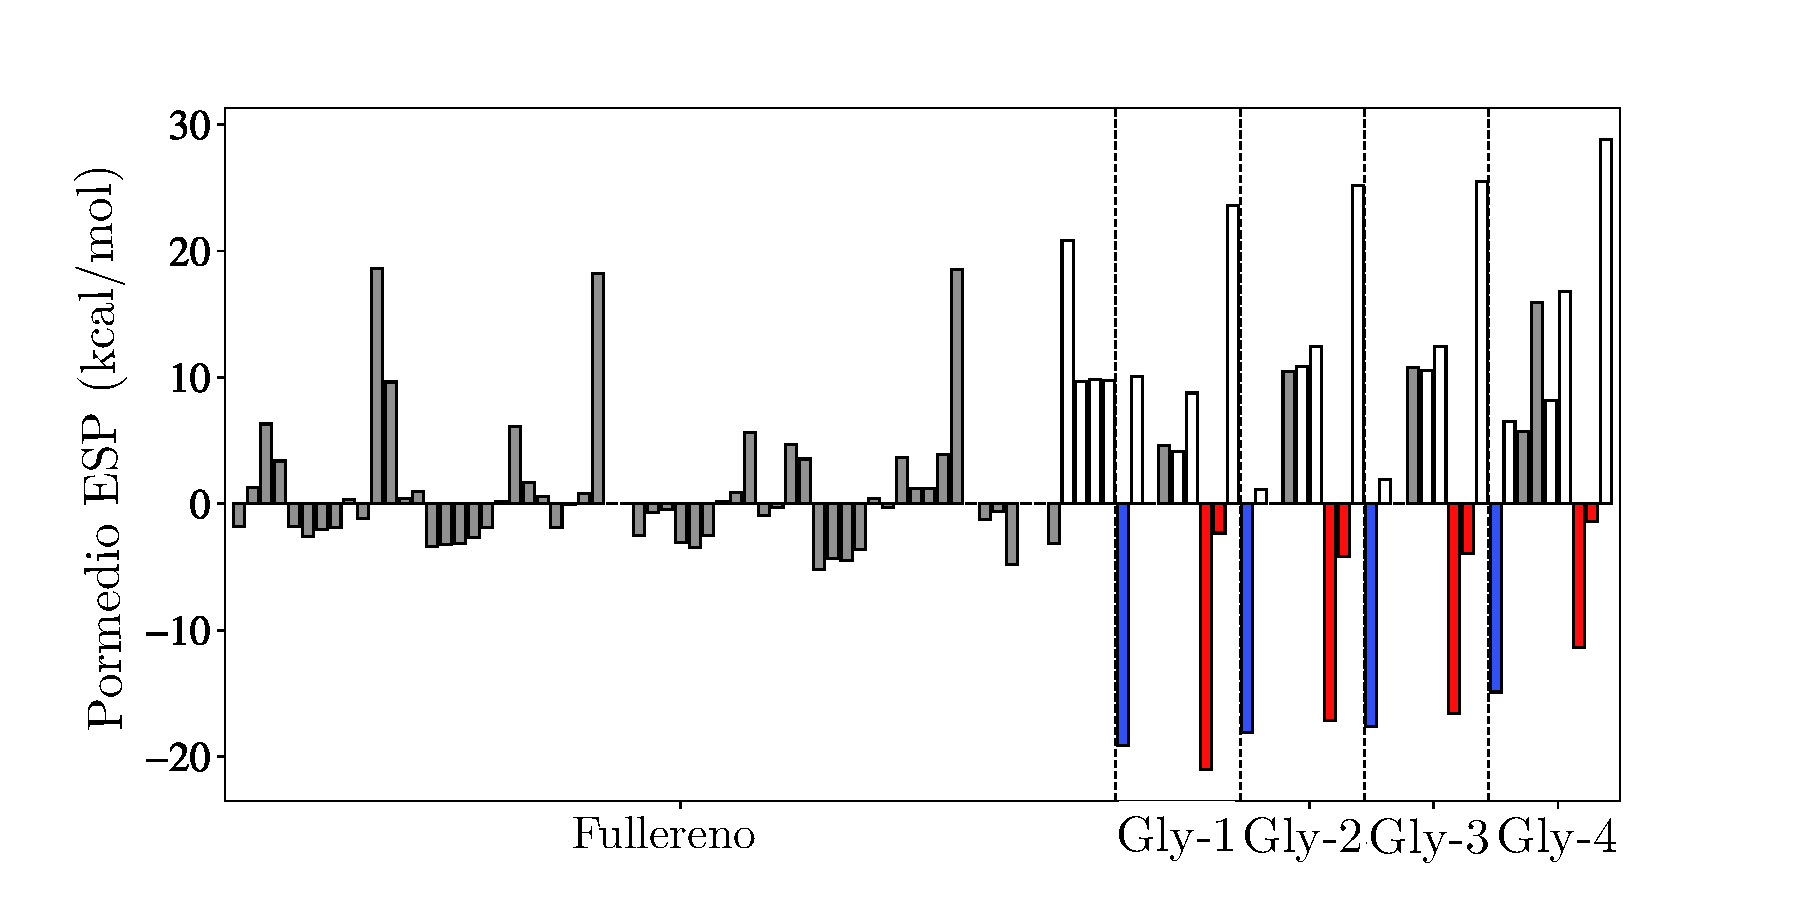
\includegraphics[width=1.0\textwidth]{imagenes/Resu/figure_2.pdf}
      \caption{Distribución de los valores de potencial electrostático promedio para el fullereno y los sistemas funcionalizados con una a cuatro glicinas. Las líneas verticales discontinuas separan cada sistema analizado.}
      \label{fig:esp-promedio}
        \end{figure}
    
    
    
                      
\begin{figure}[H]
      \centering
      \includegraphics[width=1.0\textwidth]{imagenes/Resu/figure_5.png}
      \caption{Mapa de potencial electrostático molecular del complejo C\textsubscript{60}(Gly)\textsubscript{4} observado desde dos orientaciones. La figura muestra la heterogeneidad de la superficie electrónica alrededor de la jaula de fullereno y de los grupos de glicina.}
      \label{fig:mep-gly4}
        \end{figure}
        
        
 \section{Distribución del potencial electrostático molecular (MEP)}

En la Figura~\ref{fig:esp-promedio} se presenta la distribución puntual del promedio del Potencial Electrostático (ESP, expresado en $\text{kcal mol}^{-1}$) para cada átomo del sistema, determinado mediante el software Multiwfn. 

En la jaula del fullereno prístino, los átomos de carbono muestran valores de potencial muy cercanos a cero (oscilando ligeramente en una franja neutra), lo que refleja la simetría electrónica y el carácter apolar de la red conjugada $\pi$. Sin embargo, al evaluar las adiciones secuenciales de glicina (sistemas Gly-1 a Gly-4), se evidencia una clara polarización electrónica espacial:
\begin{enumerate}
    \item \textbf{Átomos electronegativos ($O$ y $N$):} Los átomos de oxígeno y nitrógeno de los residuos de glicina presentan los potenciales más negativos del sistema, alcanzando valores mínimos de hasta $-20\text{ kcal mol}^{-1}$ (barras rojas y azules orientadas hacia abajo en la Figura~\ref{fig:esp-promedio}).
    \item \textbf{Átomos de hidrógeno polar ($H$):} Los protones pertenecientes a los grupos funcionales de la glicina exhiben los potenciales más electropositivos, superando los $+20$ y $+30\text{ kcal mol}^{-1}$ (barras dirigidas hacia arriba).
    \item \textbf{Carbonos de la jaula y grupos adyacentes:} Presentan una modulación sutil dependiendo de su cercanía a los grupos funcionales, manteniendo los carbonos de las glicinas un carácter moderadamente positivo.
\end{enumerate}

Por su parte, la Figura~\ref{fig:mep-gly4} ilustra la topografía del Mapa de Potencial Electrostático Molecular (MEP) para el complejo $C_{60}(\text{Gly})_4$ desde dos orientaciones (frente y vuelta), corroborando tridimensionalmente la heterogeneidad cuantitativa observada en la Figura~\ref{fig:esp-promedio}. La superficie molecular exhibe una marcada anfipaticidad:
\begin{itemize}
    \item \textbf{Regiones rojas (Potencial electronegativo):} Concentradas sobre los átomos de oxígeno de los carboxilos y nitrógenos, constituyendo sitios idóneos para actuar como aceptores de puentes de hidrógeno o interactuar con residuos catiónicos.
    \item \textbf{Regiones azules intensas (Potencial electropositivo):} Localizadas sobre los protones de los grupos funcionales, actuando como donadores de puentes de hidrógeno y sitios de atracción electrostática hacia residuos aniónicos.
    \item \textbf{Regiones verdes (Potencial neutro/apolar):} La superficie de la jaula de $C_{60}$ conserva una coloración verdosa dominante (potencial cercano a $0\text{ kcal mol}^{-1}$), demostrando que el núcleo no pierde su capacidad de establecer interacciones hidrofóbicas.
\end{itemize}

\subsection{Implicaciones en el reconocimiento molecular con la proteína 2FOM (DENV2)}

Esta distribución electrostática heterogénea demuestra que el aducto $C_{60}(\text{Gly})_4$ actúa como un ligando multifuncional con alta versatilidad de acoplamiento. A diferencia del fullereno prístino —cuyo mecanismo de interacción está restringido únicamente a contactos hidrofóbicos—, la tetrafuncionalización le confiere al sistema la capacidad de establecer tres tipos fundamentales de interacciones en el sitio de reconocimiento de la proteína de envoltura del virus del Dengue (DENV2, PDB ID: 2FOM):
\begin{enumerate}
    \item \textbf{Interacciones electrostáticas catiónicas:} Los lóbulos electropositivos (azules, $+30\text{ kcal mol}^{-1}$) se acoplan preferentemente con cavidades aniónicas ricas en residuos de ácido aspártico (Asp) y ácido glutámico (Glu).
    \item \textbf{Interacciones electrostáticas aniónicas:} Los lóbulos electronegativos (rojos, $-20\text{ kcal mol}^{-1}$) interactúan de manera complementaria con residuos cargados positivamente, tales como lisina (Lys), arginina (Arg) o histidina (His).
    \item \textbf{Interacciones de van der Waals y apolares:} La superficie verde neutra de la jaula permite el empaquetamiento hidrofóbico con aminoácidos aromáticos y alifáticos (como leucina, isoleucina, fenilalanina y triptófano) dentro del bolsillo catalítico o de unión de la proteína 2FOM.
\end{enumerate}

En conclusión, la funcionalización con glicina no solo mejora la solubilidad del nanomaterial, sino que genera una superficie electrónica multipolar altamente adaptable a la diversidad de aminoácidos presentes en la diana biológica 2FOM.       
        
        
        
        
        
        
        
                
\section{Acoplamiento molecular}  
La proteasa NS2B/NS3 del serotipo 2 del virus del dengue (DENV-2), con una masa molecular de $26.57\ \text{kDa}$, representa un blanco terapéutico primordial por su papel clave en la replicación viral. Al evaluar el modelo en conformación abierta e inactiva (PDB ID: \textbf{2FOM}) reconstruido en sus regiones desordenadas mediante AlphaFold, se observa que la estructura presenta una alta fidelidad conformacional.

En el mapa de Ramachandran se aprecia una distribución óptima de los ángulos diedros ($\phi, \psi$), donde la gran mayoría de los residuos se ubican en zonas energéticamente favorecidas. A partir de esta base estructural, los $100\ \text{ns}$ de dinámica molecular (MD) bajo el campo de fuerzas CHARMM36 reflejan la respuesta conformacional y la estabilidad del sistema en solución acuosa.

\begin{figure}[H]
    \centering
    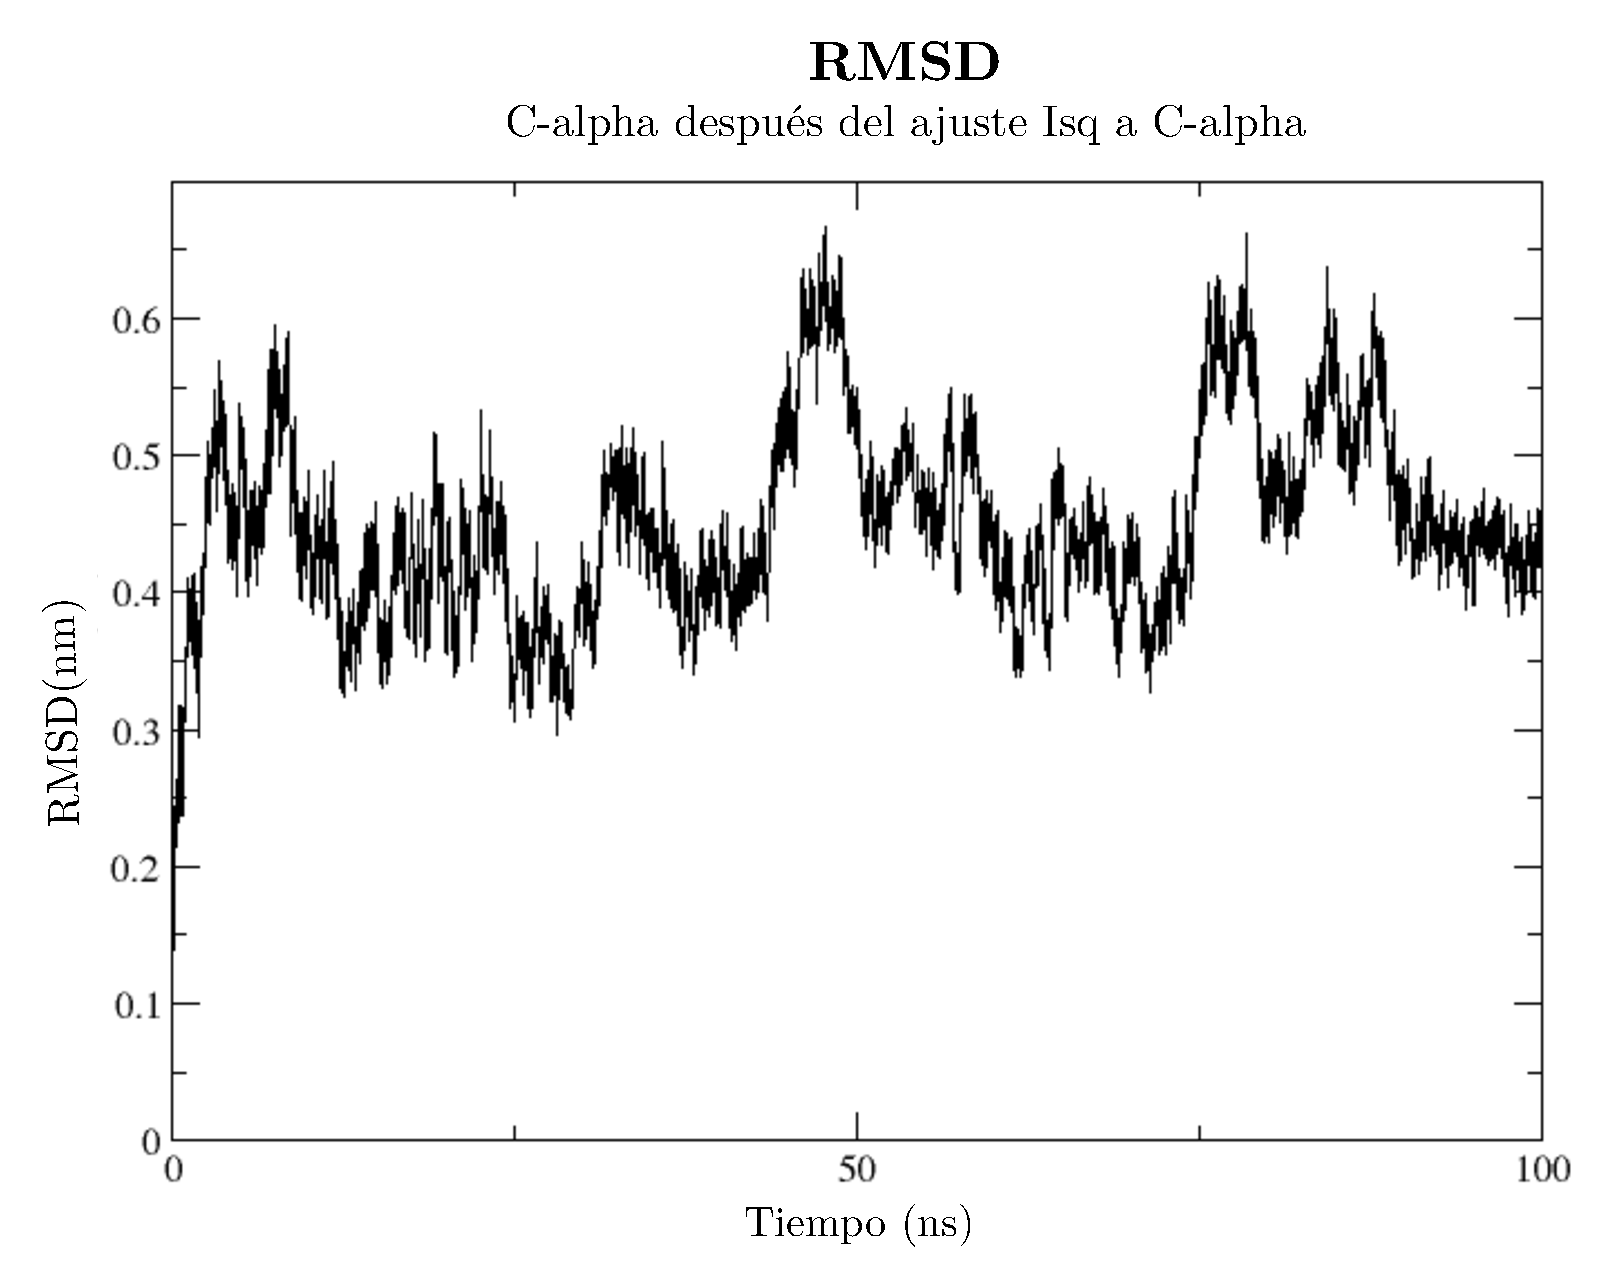
\includegraphics[width=0.82\textwidth]{imagenes/Resu/rmsd-2.pdf}
    \caption{Evolución del RMSD de los átomos C$\alpha$ de la proteína, después del ajuste por mínimos cuadrados a los átomos C$\alpha$ de referencia, durante 100 ns de dinámica molecular.}
    \label{fig:rmsd-2fom}
\end{figure}
        
\begin{figure}[H]
    \centering
    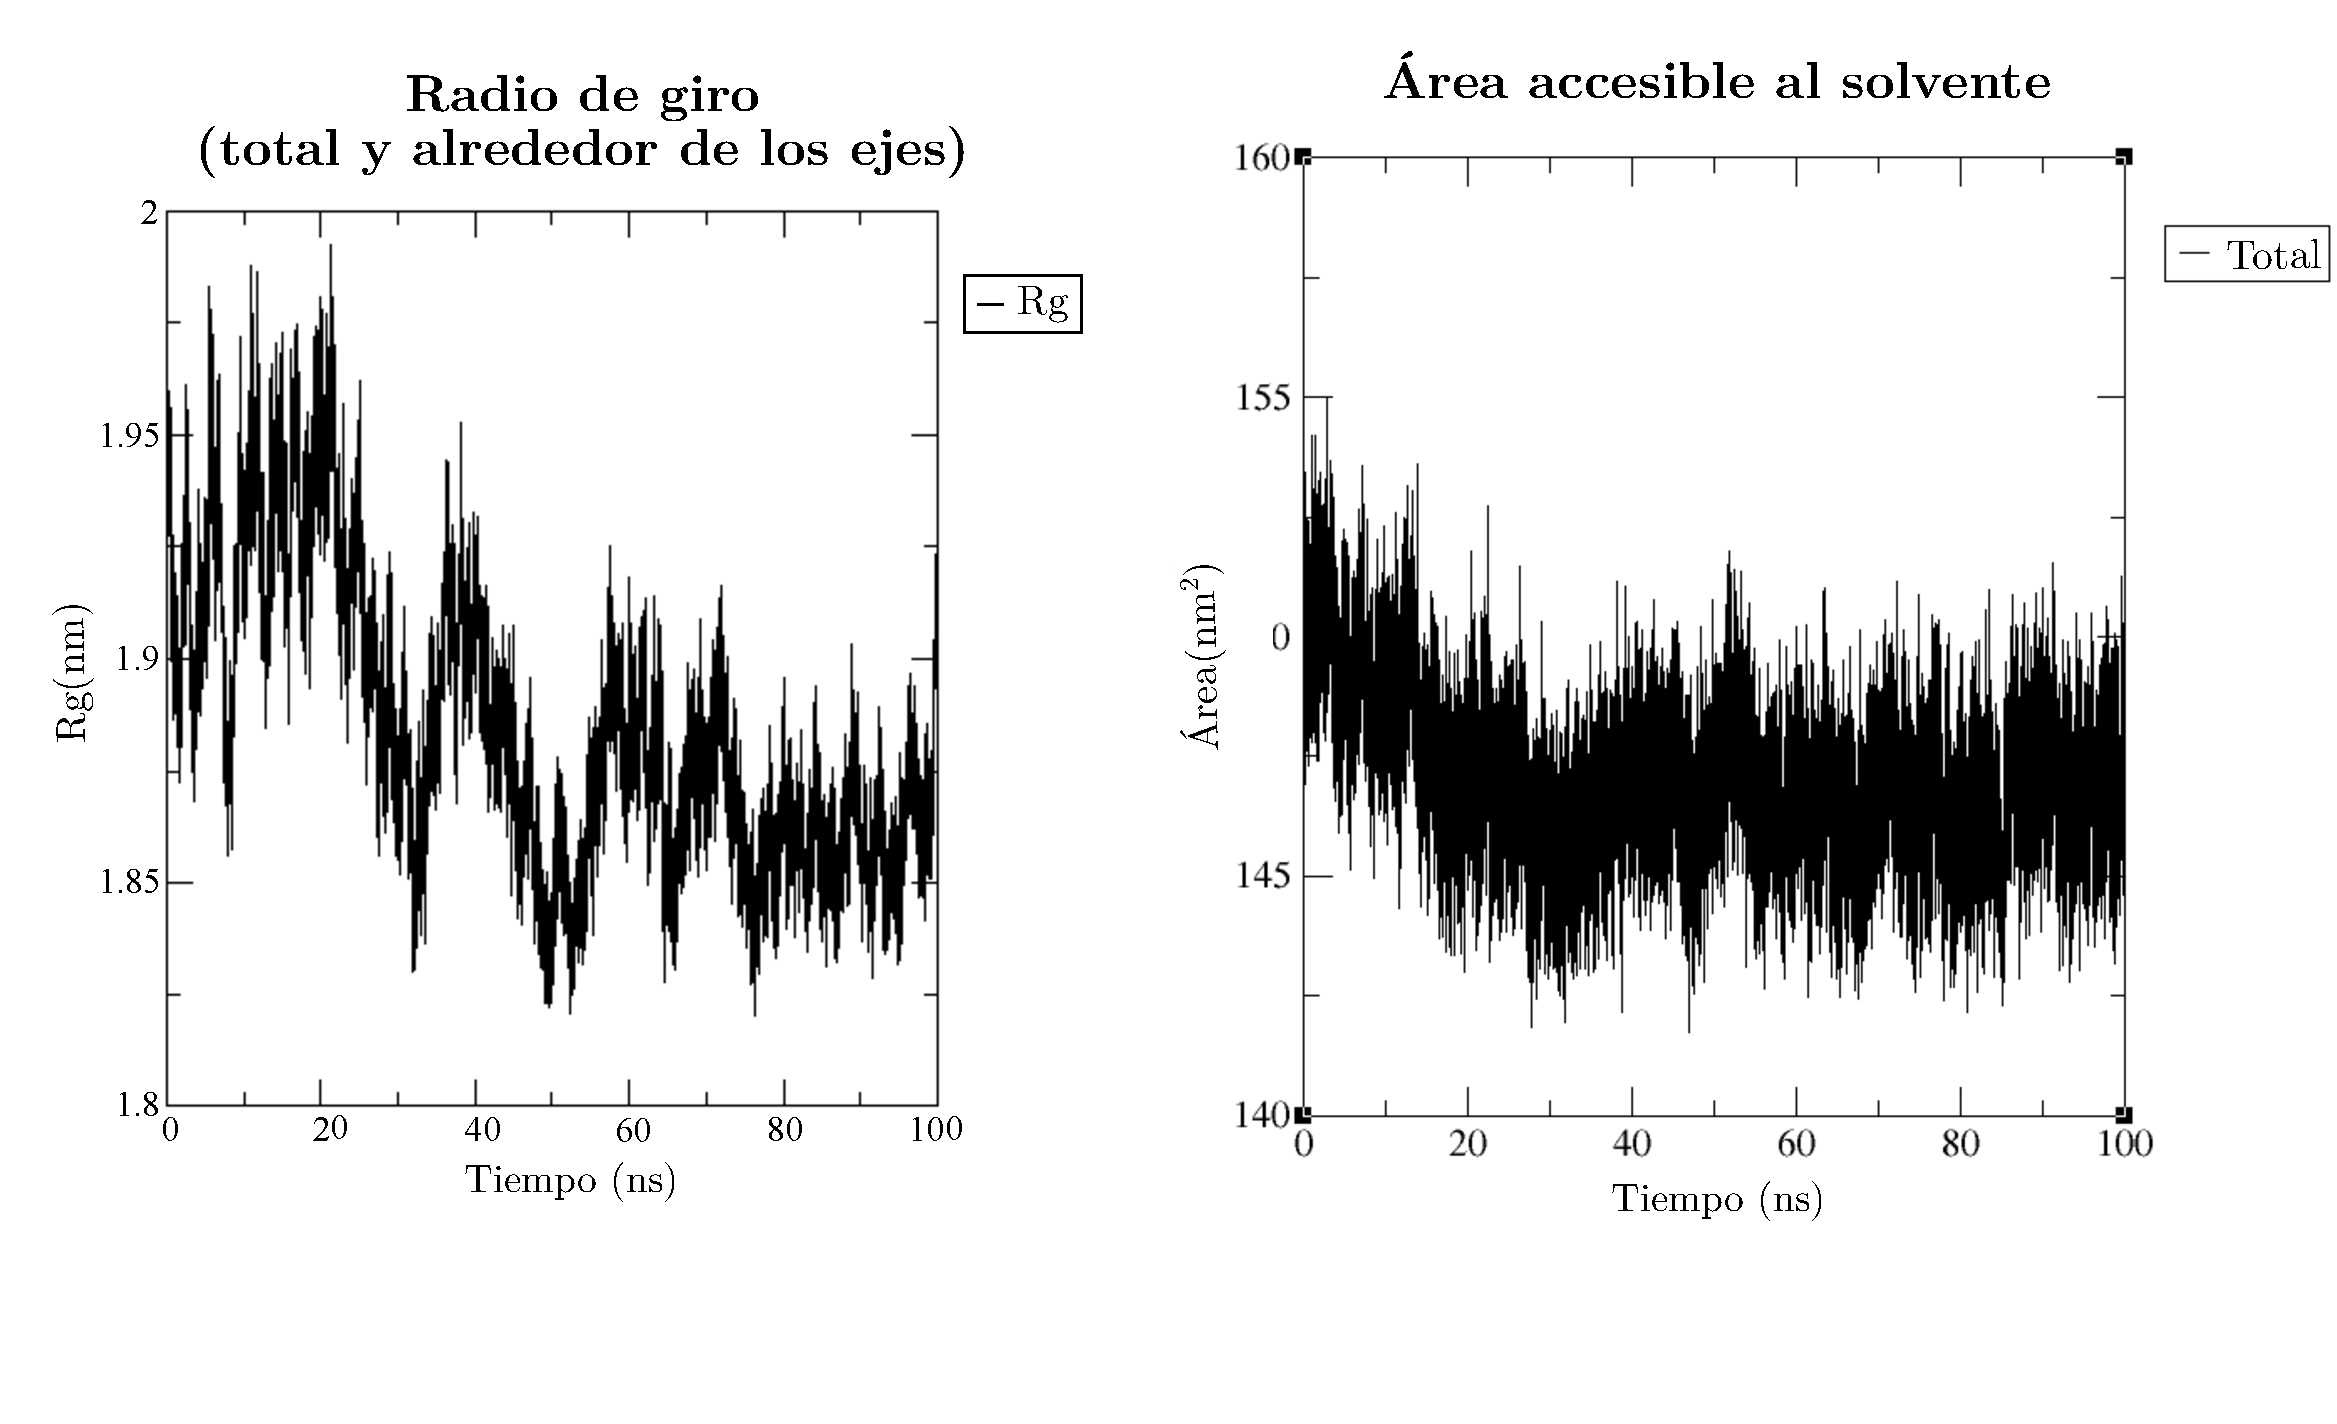
\includegraphics[width=0.95\textwidth]{imagenes/Resu/radio.pdf}
    \caption{Evolución temporal del radio de giro ($R_g$) y del área superficial accesible al solvente ($\text{SASA}$) durante los 100 ns de trayectoria de dinámica molecular.}
    \label{fig:rg-sasa-2fom}
\end{figure} 
      
\begin{figure}[H]
    \centering
    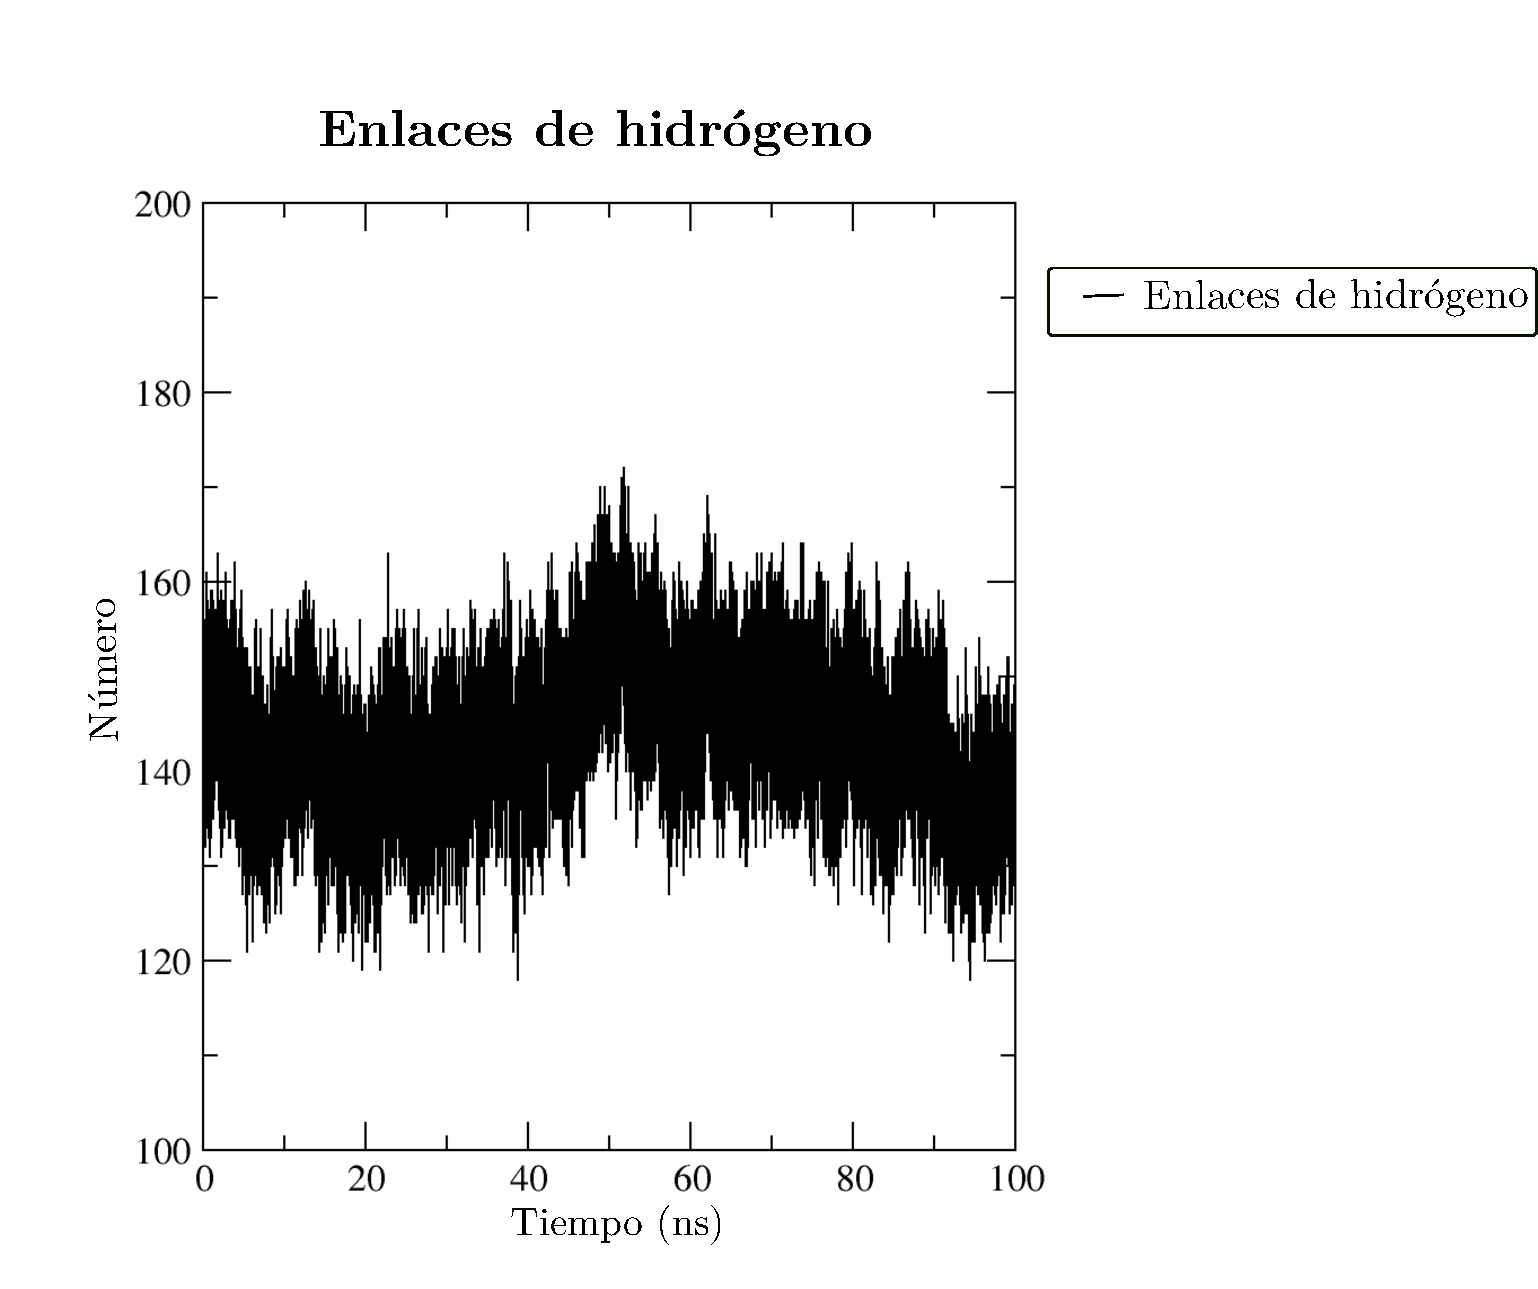
\includegraphics[width=0.70\textwidth]{imagenes/Resu/hidrogeno.pdf}
    \caption{Evolución temporal del número de enlaces de hidrógeno intramoleculares formados en la proteína a lo largo de 100 ns.}
    \label{fig:hbond-2fom}
\end{figure}   

\subsection{Comportamiento de la estabilidad global y movilidad ($\text{RMSD}$)}

Al analizar la evolución de la Desviación Cuadrática Media ($\text{RMSD}$) de los átomos $C\alpha$ (Figura~\ref{fig:rmsd-2fom}), se observa un incremento inicial rápido durante los primeros $5\ \text{ns}$ hasta alcanzar $\sim 0.40\ \text{nm}$, lo cual se atribuye a la acomodación y relajación inicial del sistema en el entorno de solvatación.

Entre los $10$ y $40\ \text{ns}$, la trayectoria exhibe un régimen de equilibrio relativo en torno a $0.40 - 0.45\ \text{nm}$. Sin embargo, entre los $45 - 55\ \text{ns}$ y $75 - 85\ \text{ns}$, se detectan fluctuaciones más marcadas que alcanzan picos de hasta $0.65\ \text{nm}$. Estas variaciones no responden a un proceso de desnaturalización, sino a la notable movilidad intrínseca de la proteína en su estado abierto e inactivo, asociada a los reordenamientos del bucle cofactórico de NS2B y del dominio catalítico. La posterior estabilización del $\text{RMSD}$ en la franja de $0.40 - 0.45\ \text{nm}$ durante los últimos $15\ \text{ns}$ confirma que el sistema convergió hacia una cuenca de energía potencial estable.

\subsection{Proceso de compactación y exposición hidrofóbica ($R_g$ y $\text{SASA}$)}

Los perfiles del Radio de Giro ($R_g$) y del Área Superficial Accesible al Solvente ($\text{SASA}$) (Figura~\ref{fig:rg-sasa-2fom}) respaldan esta interpretación y aportan información sobre el comportamiento macroestructural:

\begin{itemize}
    \item \textbf{Radio de Giro ($R_g$):} A partir del valor inicial de $1.90\ \text{nm}$, se aprecia una expansión transitoria hasta $1.97\ \text{nm}$ en los primeros $15\ \text{ns}$, producto de la apertura de bucles flexibles. No obstante, a partir del nanosegundo $20$ se identifica una tendencia continua hacia la compactación que alcanza un mínimo de $1.82\ \text{nm}$ hacia los $50\ \text{ns}$, para posteriormente mantenerse constante entre $1.84$ y $1.88\ \text{nm}$. Este comportamiento demuestra que la proteína tiende hacia un empaquetamiento más globular con el paso del tiempo.
    
    \item \textbf{Área Accesible al Solvente ($\text{SASA}$):} En concordancia con la contracción del $R_g$, se observa una disminución clara en el $\text{SASA}$ total desde $\sim 155\ \text{nm}^2$ hasta fluctuar en la franja de $145 - 150\ \text{nm}^2$. Esta reducción refleja la ocurrencia de un colapso hidrofóbico interno que minimiza la exposición de los residuos apolares al solvente.
\end{itemize}

\subsection{Dinámica de la red interna de enlaces de hidrógeno}

Al examinar la red de enlaces de hidrógeno intramoleculares (Figura~\ref{fig:hbond-2fom}), se encuentra la explicación molecular a la compactación observada. Se evidencia que la proteasa mantiene de forma constante entre $130$ y $150$ enlaces de hidrógeno internos a lo largo de toda la trayectoria. Destaca un incremento notable en la densidad de estas interacciones entre los $40$ y $60\ \text{ns}$ (con picos de hasta $\sim 165$ contactos), coincidiendo de manera exacta con el mínimo observado en el Radio de Giro ($R_g \approx 1.82\ \text{nm}$).

Este comportamiento demuestra que el fortalecimiento de la red electrostática interna actuó como la fuerza impulsora que consolidó la estructura terciaria frente a la movilidad de los bucles.

En conclusión, la consistencia observada entre la estabilización del $\text{RMSD}$ ($\sim 0.42\ \text{nm}$), la reducción del $R_g$ ($1.85\ \text{nm}$), la disminución del $\text{SASA}$ ($146\ \text{nm}^2$) y la preservación continua de la red de enlaces de hidrógeno intramoleculares permite concluir que la proteasa DENV-2 en conformación abierta e inactiva alcanza una marcada estabilidad estructural bajo las condiciones simuladas.

\begin{figure}[H]
      \centering
      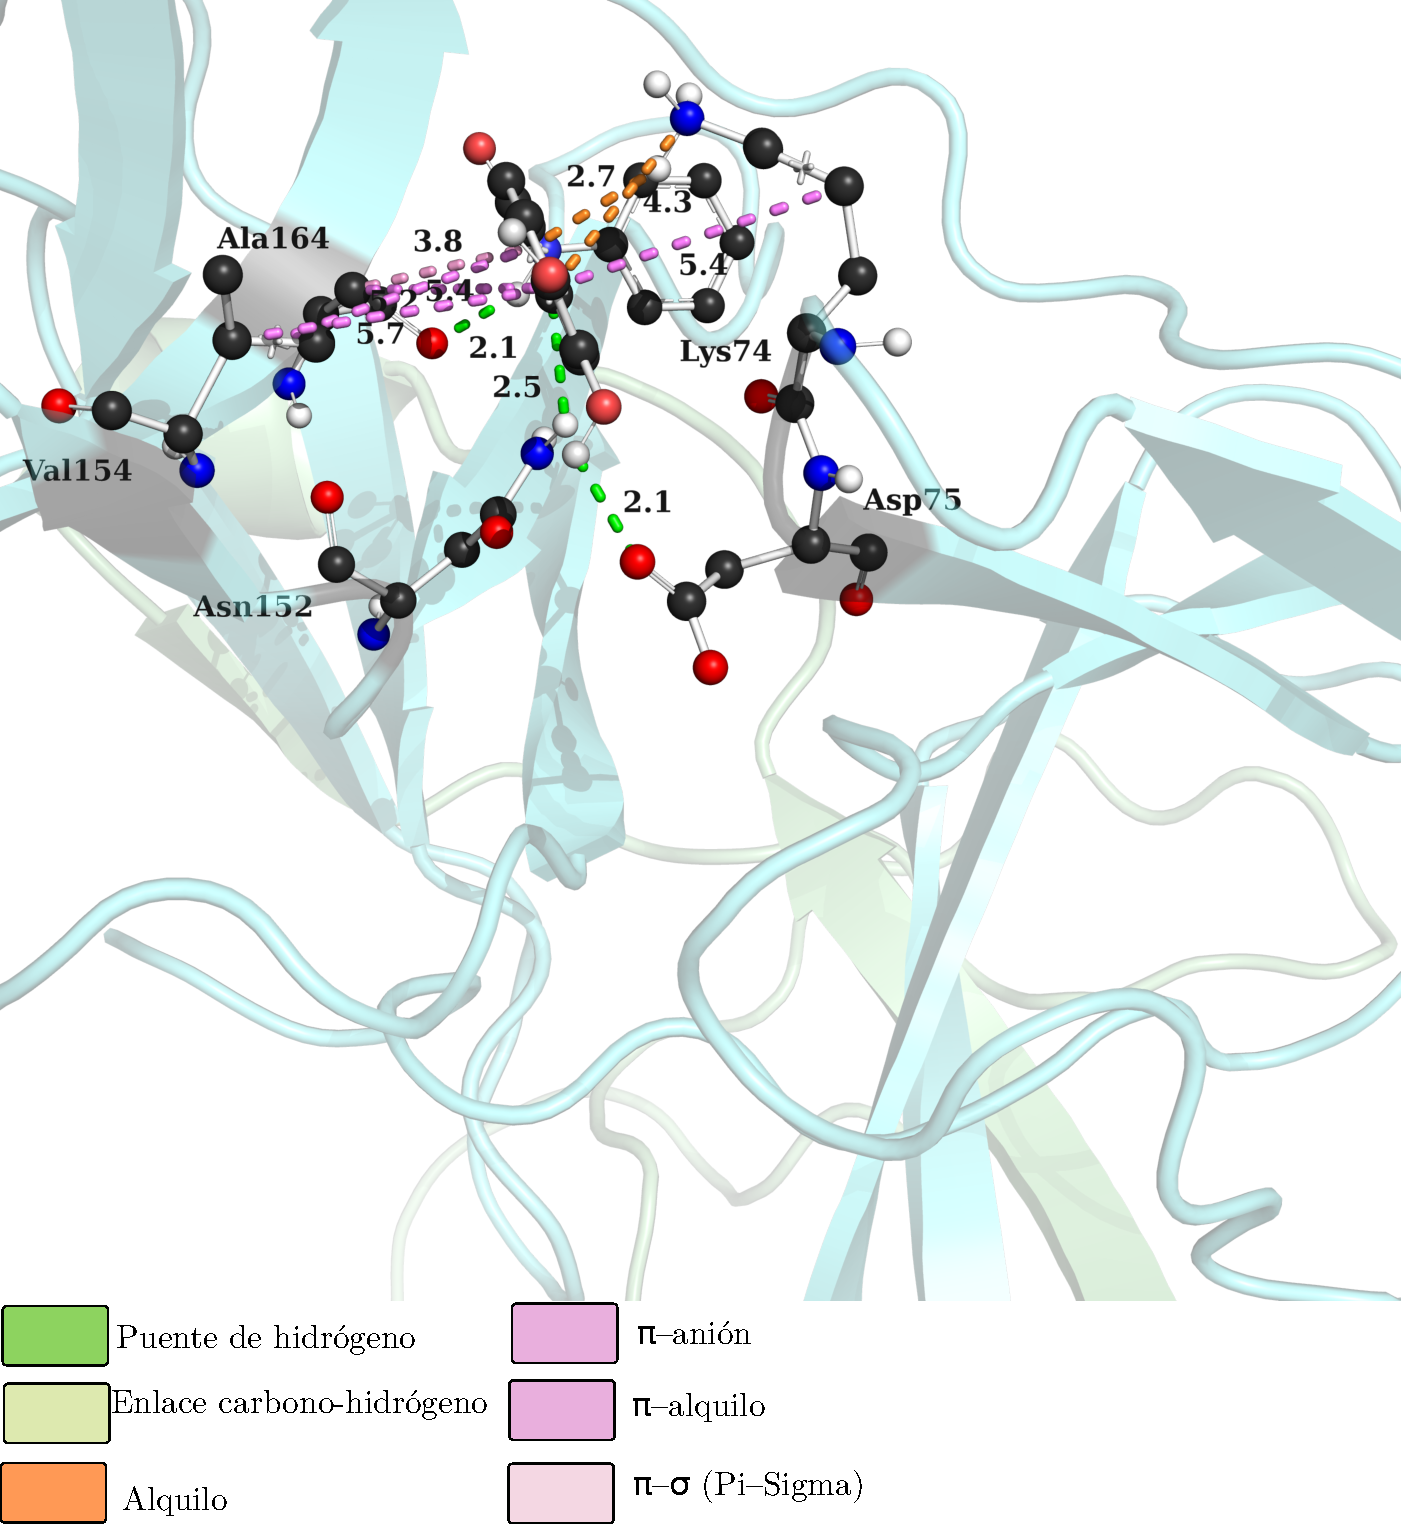
\includegraphics[width=1.0\textwidth]{imagenes/Resu/benza.pdf}
      \caption{Representación 3D del acoplamiento molecular del derivado benzamida en la cavidad alostérica de la proteasa de DENV-2 (Pose 61). Se presentan las distancias de enlace expresadas en ångströms (\AA).}
      \label{fig:mep-gly4}
        \end{figure}

\begin{figure}[H]
      \centering
      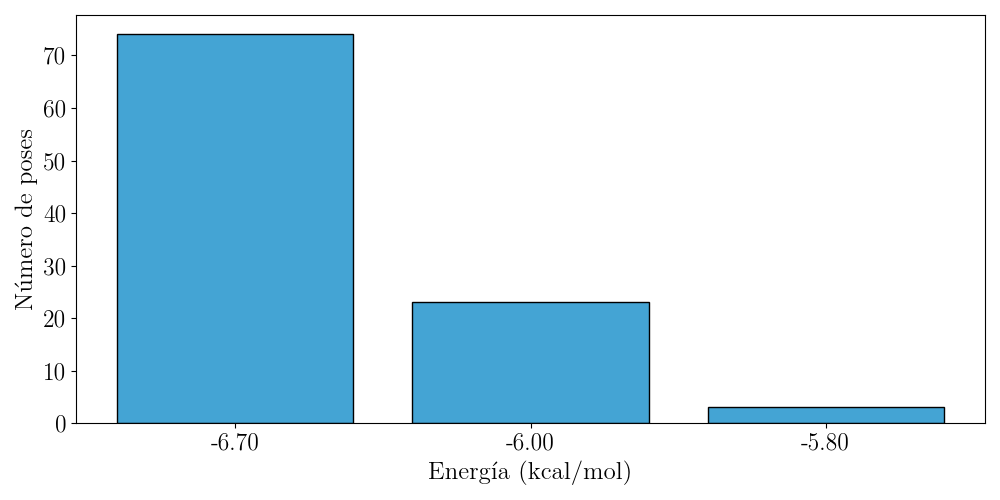
\includegraphics[width=1.0\textwidth]{imagenes/Resu/benza-3.png}
      \caption{M.}
      \label{fig:mep-gly4}
        \end{figure}
        
 \begin{table}[H]
    \centering
    \footnotesize % Tamaño de letra más pequeño para que entre holgadamente
    \setlength{\tabcolsep}{5pt} % Otorga espacio entre columnas para que no se peguen
    \renewcommand{\arraystretch}{1.2}
    \caption{Interacciones no covalentes y distancias de contacto para el acoplamiento del inhibidor alostérico derivado de benzamida en la proteasa de DENV-2 (PDB: 2FOM).}
    \label{tab:interacciones-2fom}
    \begin{tabular}{llcll}
        \toprule
        \multicolumn{1}{c}{\textbf{\shortstack[c]{Tipo de\\interacción}}} & 
        \multicolumn{1}{c}{\textbf{Residuo}} & 
        \multicolumn{1}{c}{\textbf{\shortstack[c]{Distancia\\(\AA)}}} & 
        \multicolumn{1}{c}{\textbf{\shortstack[c]{Motivo\\estructural}}} & 
        \multicolumn{1}{c}{\textbf{\shortstack[c]{Tipo de\\aminoácido}}} \\
        \midrule
        Puente de hidrógeno & Ala164 & 2.07 & Sitio de unión & Apolar / Hidrofóbico \\
                            & Asn152 & 2.52 & Sitio de unión & Polar no cargado \\
                            & Asp75  & 2.12 & Tríada catalítica & Polar, cargado negativo \\
        \midrule
        $\pi$-Catión        & Lys74  & 2.62 & Bolsillo S1 / Sitio activo & Polar, cargado positivo \\
                            & Lys74  & 4.27 & Bolsillo S1 / Sitio activo & Polar, cargado positivo \\
        \midrule
        Interacción hidrofóbica & Val154 & 4.91 & Bolsillo hidrofóbico & Apolar / Hidrofóbico \\
                                & Val154 & 5.16 & Bolsillo hidrofóbico & Apolar / Hidrofóbico \\
                                & Val154 & 5.40 & Bolsillo hidrofóbico & Apolar / Hidrofóbico \\
        \bottomrule
    \end{tabular}
\end{table}
      Se seleccionó la conformación de menor energía ($-6.00 \text{ kcal/mol}$) por presentar el anclaje mediante puente de hidrógeno con el residuo Gly133 del hueco oxianiónico, permitiendo evaluar mediante Dinámica Molecular la estabilidad temporal de esta interacción. 

con un limite de 5.0 y una exaustividad de 80, -6.70 kcal/mol con 74 modelos, otra con -5.80 kcal/mol con 3 modelos y -6.00 kcal/mol con 23 modelos, segun la literatura, estos son los sitios donde se une. 

Como se observa en el perfil energético de la Figura~9.11, el acoplamiento molecular exhibió una marcada convergencia conformacional. La conformación de menor energía libre de unión alcanzó un valor de $-6.70\ \text{kcal/mol}$, concentrando un 74\% del total de las poses generadas. Destacando la estabilidad del complejo ligando-proteína y sugiere que el modo de unión es una pose termodinámicamente favorable en el bolsillo alostérico.
Al contrastar los contactos atómicos obtenidos (Tabla~9.5 y Figura~2D/3D) con los hallazgos reportados en la literatura para inhibidores alostéricos de estructura similar (como el derivado de benzofurano 34e, $\text{IC}_{50} = 0.69\ \mu\text{M}$), se identifican importantes coincidencias estructurales y mecanísticas:

\begin{itemize}
    \item \textbf{Red de Puentes de Hidrógeno y el ``Interruptor Molecular'' (\textbf{Asn152}):} En nuestros resultados, el oxígeno del anillo de benzofurano establece un puente de hidrógeno convencional con la cadena lateral de \textbf{Asn152} a una distancia de $2.52\ \text{\AA}$. Este hallazgo es de vital relevancia, ya que la literatura señala a \textbf{Asn152} como un ``interruptor molecular'' clave responsable de mantener a la enzima en su conformación inactiva. Adicionalmente, el grupo hidroxilo del anillo aromático forma un puente de hidrógeno fuerte de $2.12\ \text{\AA}$ con \textbf{Asp75} (perteneciente a la tríada catalítica), mientras que el grupo N--H de la amida interactúa mediante un enlace de hidrógeno de $2.07\ \text{\AA}$ con el esqueleto de \textbf{Ala164}. Esta red tripartita de puentes de hidrógeno ancla firmemente el ligando al sitio de unión.
    
    \item \textbf{Interacciones Electrostáticas y $\pi$-Catiónicas con \textbf{Lys74}:} La literatura reporta que en derivados como el 34e, la orientación inclinada (\textit{tilted}) del núcleo aromático y el carbonilo amídico permite una interacción crítica con \textbf{Lys74}. En nuestros cálculos de \textit{docking}, se confirmó la participación activa de este residuo mediante dos interacciones de tipo $\pi$-catión con el sistema aromático del compuesto a distancias de $2.62\ \text{\AA}$ y $4.27\ \text{\AA}$. Esta atracción electrostática refuerza la fijación del andamio (\textit{scaffold}) en la entrada del bolsillo S1/alostérico.
    
    \item \textbf{Complementariedad en el Subbolsillo Hidrofóbico:} El análisis de contactos no polares reveló interacciones de tipo $\pi$-sigma y $\pi$-alquil entre el sistema aromático y el residuo \textbf{Val154} ($4.91\ \text{\AA}$, $5.16\ \text{\AA}$ y $5.40\ \text{\AA}$). Aunque los estudios reportados previamente destacan la inserción lipofílica hacia residuos como \textbf{Leu76}, \textbf{Gly148} e \textbf{Ile165}, el contacto hallado con \textbf{Val154} demuestra una acomodación hidrofóbica equivalente que estabiliza el núcleo aromático dentro de la cavidad no polar.
\end{itemize}

Los datos \textit{in silico} obtenidos respaldan el mecanismo de inhibición alostérica no competitiva previamente sustentado por estudios cinéticos ($K_i$) y de mutagénesis dirigida (T122C). Al alojarse en la cavidad posterior cerca del residuo \textbf{Thr122} e interactuar directamente con la tríada catalítica (\textbf{Asp75}) y los residuos de control conformacional (\textbf{Asn152} y \textbf{Lys74}), el ligando bloquea la flexibilidad funcional requerida para el procesamiento del sustrato poliproteico.

En conjunto, la consistencia entre los valores de energía observados, la baja distancia de los puentes de hidrógeno ($\le 2.52\ \text{\AA}$) y la concordancia con los residuos clave descritos en la literatura ratifican la efectividad del \textit{scaffold} evaluado como un candidato promisorio para el desarrollo de fármacos antivirales selectivos contra DENV-2.
 
 \begin{figure}[H]
      \centering
      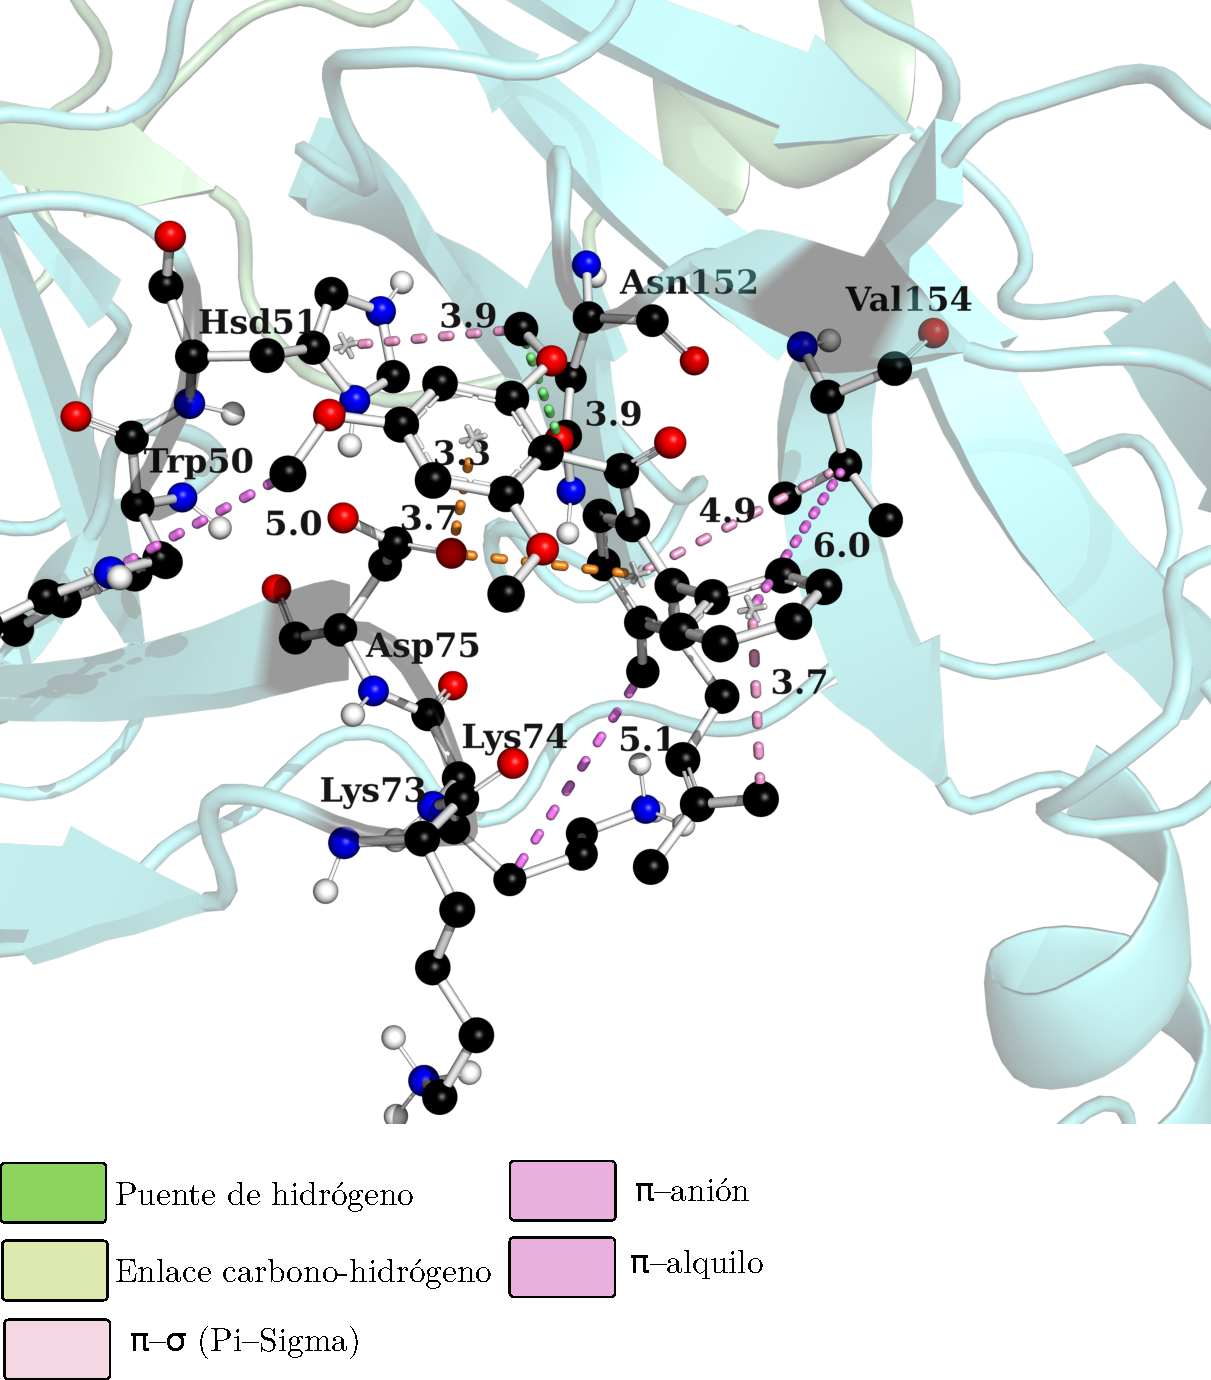
\includegraphics[width=1.0\textwidth]{imagenes/Resu/246.pdf}
      \caption{Representación 3D del acoplamiento molecular del derivado 246D  en la cavidad ortostérica de la proteasa de DENV-2 (Pose 03). Se presentan las distancias de enlace expresadas en ångströms (\AA).}
      \label{fig:mep-gly4}
        \end{figure}
       
\begin{figure}[H]
      \centering
      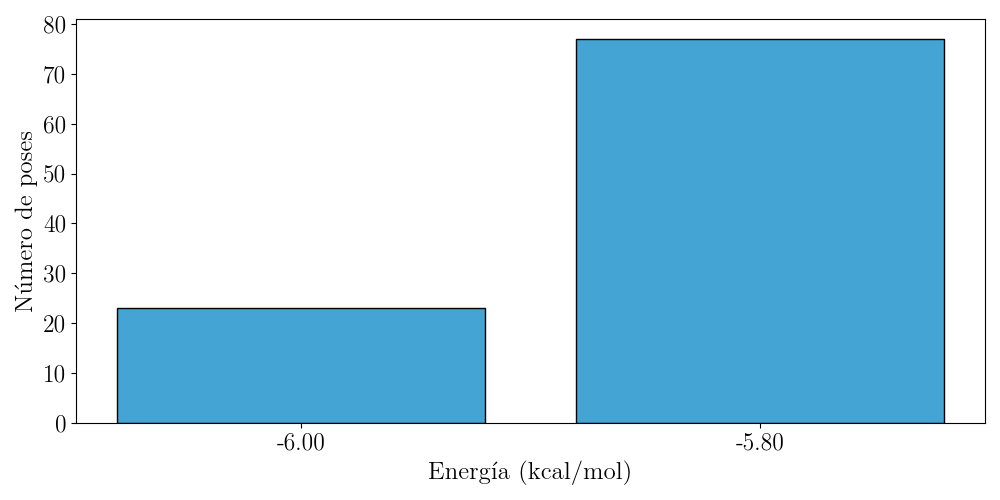
\includegraphics[width=1.0\textwidth]{imagenes/Resu/246-1.png}
      \caption{M.}
      \label{fig:mep-gly4}
        \end{figure}

  \begin{table}[H]
    \centering
    \footnotesize
    \setlength{\tabcolsep}{5pt}
    \renewcommand{\arraystretch}{1.2}
    \caption{Interacciones no covalentes y distancias de contacto para el acoplamiento del inhibidor orto 264 en la proteína de DENV-2 (PDB: 2FOM).}
    \label{tab:interacciones-pose83}
    \begin{tabular}{llcll}
        \toprule
        \multicolumn{1}{c}{\textbf{\shortstack[c]{Tipo de\\interacción}}} & 
        \multicolumn{1}{c}{\textbf{Residuo}} & 
        \multicolumn{1}{c}{\textbf{\shortstack[c]{Distancia\\(\AA)}}} & 
        \multicolumn{1}{c}{\textbf{\shortstack[c]{Motivo\\estructural}}} & 
        \multicolumn{1}{c}{\textbf{\shortstack[c]{Tipo de\\aminoácido}}} \\
        \midrule
        Enlace de H de carbono & Asn152 & 3.76 & Sitio de unión & Polar no cargado \\
        \midrule
        $\pi$-Anión            & Asp75  & 3.28 & Tríada catalítica & Polar, cargado negativo \\
                               & Asp75  & 3.88 & Tríada catalítica & Polar, cargado negativo \\
        \midrule
        $\pi$-Sigma            & Val154 & 3.07 & Bolsillo hidrofóbico & Apolar / Hidrofóbico \\
                               & Hsd51  & 3.85 & Tríada catalítica & Polar, cargado positivo \\
        \midrule
        Interacción hidrofóbica & Trp50  & 4.03 & Bolsillo hidrofóbico & Apolar / Aromático \\
        (Alquil / $\pi$-Alquil) & Lys74  & 4.42 & Bolsillo S1 / Sitio activo & Polar, cargado positivo \\
                               & Val154 & 4.72 & Bolsillo hidrofóbico & Apolar / Hidrofóbico \\
                               & Val154 & 5.32 & Bolsillo hidrofóbico & Apolar / Hidrofóbico \\
        \bottomrule
    \end{tabular}
\end{table}




El análisis del acoplamiento molecular realizado mediante el programa AutoDock Vina (configurado con una exhaustividad de 80) permitió evaluar la afinidad y el modo de unión del ligando en el sitio catalítico del receptor. A partir de una muestra de 100 poses generadas, el perfil energético reveló la presencia de dos conformaciones principales: un primer grupo de 23 poses con una energía libre de unión de $-6.00\ \text{kcal/mol}$ y un segundo conglomerado (\textit{cluster}) predominante correspondiente a 77 poses con una energía de $-5.80\ \text{kcal/mol}$ (Figura~9.1.b).

A pesar de que el primer grupo presentó el valor de energía mínimo absoluto, la selección final del modo de acoplamiento recayó en la \texttt{pose03.pdb} (perteneciente al \textit{cluster} de $-5.80\ \text{kcal/mol}$). Esta decisión se fundamenta en un criterio estadístico y termodinámico: la representación poblacional del 77\% sugiere una mayor probabilidad de ocurrencia del estado conformacional en equilibrio. Además, la diferencia energética de apenas $\Delta E = 0.2\ \text{kcal/mol}$ entre ambos mínimos se encuentra bien dentro del margen del ruido térmico ($k_B T \approx 0.6\ \text{kcal/mol}$ a temperatura ambiente), lo que demuestra que ambas poses son energéticamente equivalentes pero la \texttt{pose03.pdb} es representativa de la microconformación más probable.

La inspección visual y la caracterización de los contactos no covalentes efectuada en PyMOL y Discovery Studio Visualizer (Cuadro~9.5 y Figura~9.1.3) permitieron identificar el patrón de interacciones que estabiliza dicho complejo:

\begin{itemize}
    \item \textbf{Enlaces de Carbono-Hidrógeno y contactos polares:} Se observaron interacciones fuertemente estabilizadoras mediadas por enlaces de carbono-hidrógeno, destacando el papel del residuo polar no cargado \textbf{Asn152}. Este residuo actúa como un ancla clave en la cavidad al interaccionar directamente con los átomos de carbono-hidrógeno del ligando a distancias cortas de contacto.
    \item \textbf{Interacciones electrostáticas y relativas a electrones $\pi$:} Se identificaron interacciones del tipo $\pi$-anión y $\pi$-sigma con los residuos de la tríada catalítica y del contorno del sitio activo (\textbf{His51}, \textbf{Asp75} y \textbf{Lys74}), así como contactos hidrofóbicos ($\pi$-alquilo / alquilo) con residuos como \textbf{Val154} y \textbf{Trp50}.
\end{itemize}

Al contrastar nuestros resultados con el estudio de referencia reportado por literatura para el inhibidor sintético 246DA ($K_i = 19.84\ \mu\text{M}$) acoplado en la proteasa NS2B/NS3 del serotipo 2 del virus del dengue (PDB ID: \textbf{2FOM}, resolución de $1.5\ \text{\AA}$), se observa una coincidencia estructural y funcional sobresaliente. En la literatura se reporta que la potencia del compuesto 246DA radica en su capacidad para interaccionar mediante puentes de hidrógeno directos con la tríada catalítica (\textbf{His51}, \textbf{Asp75} y \textbf{Ser135}), a la vez que ocupa el bolsillo hidrofóbico coordinándose con residuos como \textbf{Leu76}, \textbf{Trp83}, \textbf{Ile165} e \textbf{Ile166}. 

Nuestras observaciones reafirman que la \texttt{pose03.pdb} adopta una orientación tridimensional coherente con dicho modelo bioactivo. Aunque nuestro acoplamiento con AutoDock Vina prioriza las fuerzas de Van der Waals, electrostáticas y enlaces C--H con residuos como \textbf{Asn152}, \textbf{His51} y \textbf{Asp75}, la conservación del anclaje en los residuos de la tríada catalítica confirma la validez biológica del acoplamiento. Esto sugiere que el complejo obtenido reproduce los requerimientos farmacofóricos necesarios para la inhibición competitiva de la proteasa viral DEN2.
    
\begin{figure}[H]
      \centering
      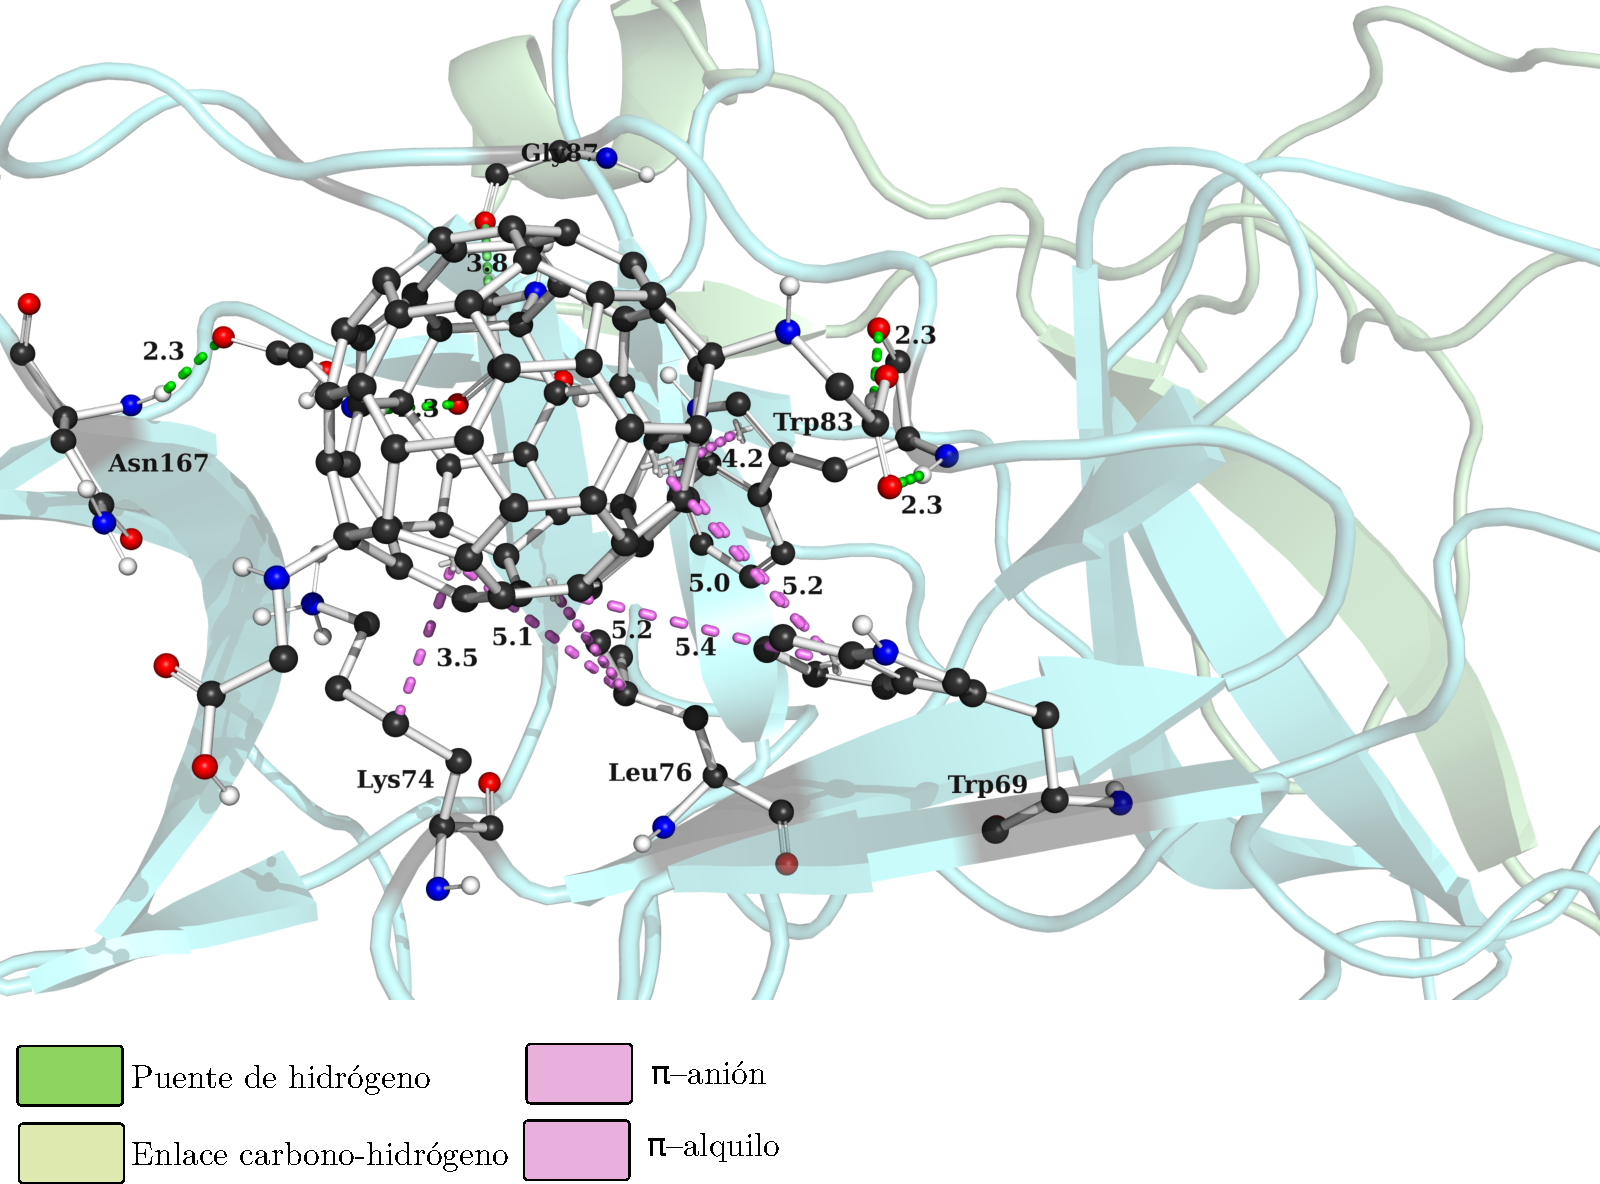
\includegraphics[width=1.0\textwidth]{imagenes/Resu/ciego.pdf}
      \caption{M.}
      \label{fig:mep-gly4}
        \end{figure}
        
\begin{figure}[H]
      \centering
      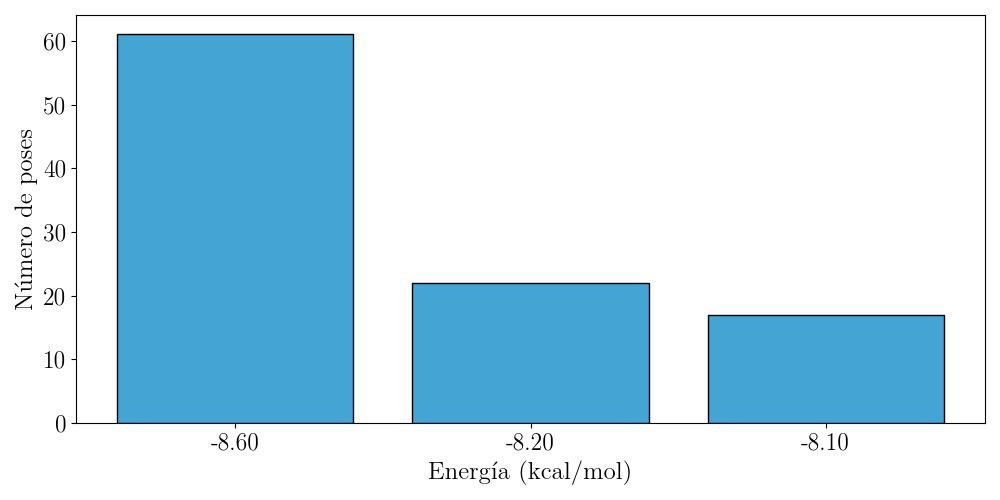
\includegraphics[width=1.0\textwidth]{imagenes/Resu/ciego.png}
      \caption{M.}
      \label{fig:mep-gly4}
        \end{figure}
        
   \begin{table}[H]
    \centering
    \footnotesize
    \setlength{\tabcolsep}{5pt}
    \renewcommand{\arraystretch}{1.2}
    \caption{Interacciones no covalentes y distancias de contacto para el acoplamiento ciego del derivado de fullereno C\textsubscript{60}(Gly)\textsubscript{4} en la proteasa de DENV-2 (PDB: 2FOM, Pose 72).}
    \label{tab:interacciones-pose72}
    \begin{tabular}{llcll}
        \toprule
        \multicolumn{1}{c}{\textbf{\shortstack[c]{Tipo de\\interacción}}} & 
        \multicolumn{1}{c}{\textbf{Residuo}} & 
        \multicolumn{1}{c}{\textbf{\shortstack[c]{Distancia\\(\AA)}}} & 
        \multicolumn{1}{c}{\textbf{\shortstack[c]{Motivo\\estructural}}} & 
        \multicolumn{1}{c}{\textbf{\shortstack[c]{Tipo de\\aminoácido}}} \\
        \midrule
        Puente de hidrógeno & Lys74  & 2.92 & Bolsillo S1 / Sitio activo & Polar, cargado positivo \\
        \midrule
        Enlace de H de carbono & Asp174 & 3.26 & Sitio de unión & Polar, cargado negativo \\
                            & Asn167 & 3.40 & Sitio de unión & Polar no cargado \\
                            & Gly48 & 3.78 & Sitio de unión & Apolar / Neutro \\
        \midrule
        Interacción hidrofóbica & Trp83  & 5.24 & Bolsillo hidrofóbico & Apolar / Aromático \\
        ($\pi$-Alquil) & & & & \\
        \bottomrule
    \end{tabular}
\end{table}
     El análisis del acoplamiento ciego (\textit{blind docking}) realizado mediante el programa AutoDock Vina permitió evaluar la capacidad de interacción, la afinidad termodinámica y el modo de unión del derivado de fulereno tetra-aducto de glicina (C\textsubscript{60}(Gly)\textsubscript{4}) sobre la estructura tridimensional de la proteasa NS2B/NS3 del serotipo 2 del virus del dengue (PDB ID: \textbf{2FOM}). A partir de un muestreo de 100 poses generadas, el perfil energético reveló una distribución conformacional dividida en tres conglomerados (\textit{clusters}) principales: un primer grupo mayoritario de 61 poses con una energía libre de unión ($\Delta G$) de $-8.60\ \text{kcal/mol}$, seguido de un segundo grupo de 22 poses con $-8.20\ \text{kcal/mol}$ y un tercer grupo de 17 poses con $-8.10\ \text{kcal/mol}$ (Figura~9.16).

La selección del modo de acoplamiento óptimo recayó en la \texttt{pose72.pdb}, perteneciente al \textit{cluster} con el mínimo energético absoluto de $-8.60\ \text{kcal/mol}$. A diferencia de sistemas donde el mínimo energético y la densidad conformacional divergen, en este caso coinciden ambos criterios: la amplia representación poblacional (61\%) demuestra que esta conformación no solo es la más estable termodinómicamente, sino también  en equilibrio más probable durante el proceso de reconocimiento molecular. Asimismo, el valor atrayente de $-8.60\ \text{kcal/mol}$ refleja una afinidad sustancialmente elevada, favorecida por la naturaleza anfífilica del aducto, el cual combina el núcleo hidrofóbico del fulereno $C_{60}$ con las cadenas polares de glicina.

La caracterización detallada de los contactos no covalentes efectuada mediante PyMOL y Discovery Studio Visualizer (Tabla~9.7 e Ilustración visual) permitió dilucidar el patrón de interacciones responsables de la estabilización del complejo nanoestructura-proteína:

\begin{itemize}
    \item \textbf{Puentes de hidrógeno convencionales:} Se identificó un puente de hidrógeno fuerte entre el grupo carboxilo/amino de las cadenas de glicina del ligando y el residuo \textbf{Lys74} a una distancia de $2.92\ \text{\AA}$. Este contacto en el subsitio S1 / entorno del sitio activo actúa como un ancla electrostática y polar determinante para la orientación del aducto.
    \item \textbf{Enlaces de hidrógeno no convencionales (C--H):} Se detectaron interacciones estabilizadoras débiles tipo $\text{C--H}\cdots\text{O/N}$ con los residuos \textbf{Asp174} ($3.26\ \text{\AA}$), \textbf{Asn167} ($3.40\ \text{\AA}$) y \textbf{Gly48} ($3.78\ \text{\AA}$), las cuales contribuyen a fijar los sustituyentes de glicina a lo largo del contorno de la cavidad de unión.
    \item \textbf{Interacciones hidrofóbicas ($\pi$-Alquil):} El núcleo aromático de la esfera de fulereno establece contactos lipofílicos de tipo $\pi$-alquilo con el residuo aromático \textbf{Trp83} a una distancia de $5.24\ \text{\AA}$, acomodándose adecuadamente dentro del bolsillo hidrofóbico de la proteasa.
\end{itemize}

Al contrastar estos resultados con la literatura reportada para aductos de fulereno-glicina (C\textsubscript{60}(Gly)), se constata una consistencia notable con las propiedades fisicoquímicas y de unión a proteínas descritas experimentalmente. En estudios previos se ha demostrado mediante calorimetría de titulación isotérmica (ITC) que los aductos de C\textsubscript{60}(Gly) presentan una elevada constante de asociación con proteínas séricas humanas ($K_b = 1.3 \times 10^6\ \text{M}^{-1}$), impulsada principalmente por fuerzas hidrofóbicas y solvatación favorable, sin generar efectos citotóxicos ni genotóxicos significativos. De manera análoga, nuestros resultados \textit{in silico} confirman que el C\textsubscript{60}(Gly)\textsubscript{4} posee la versatilidad estructural para insertarse en la cavidad catalítica de la proteasa DEN2 (PDB ID: \textbf{2FOM}), acoplándose simultáneamente al subsitio S1 (\textbf{Lys74}) y al bolsillo hidrofóbico (\textbf{Trp83}).

En conjunto, la conservación de estos anclajes clave y la alta afinidad calculada sugerirían que la \texttt{pose72.pdb} logra ocluir estéricamente el sitio activo de la proteasa NS2B/NS3, validando la hipótesis de que el derivado C\textsubscript{60}(Gly)\textsubscript{4} se comporta como un potencial inhibidor competitivo o nano-plataforma bioactiva contra el virus del dengue serotipo 2.
        
\begin{figure}[H]
      \centering
      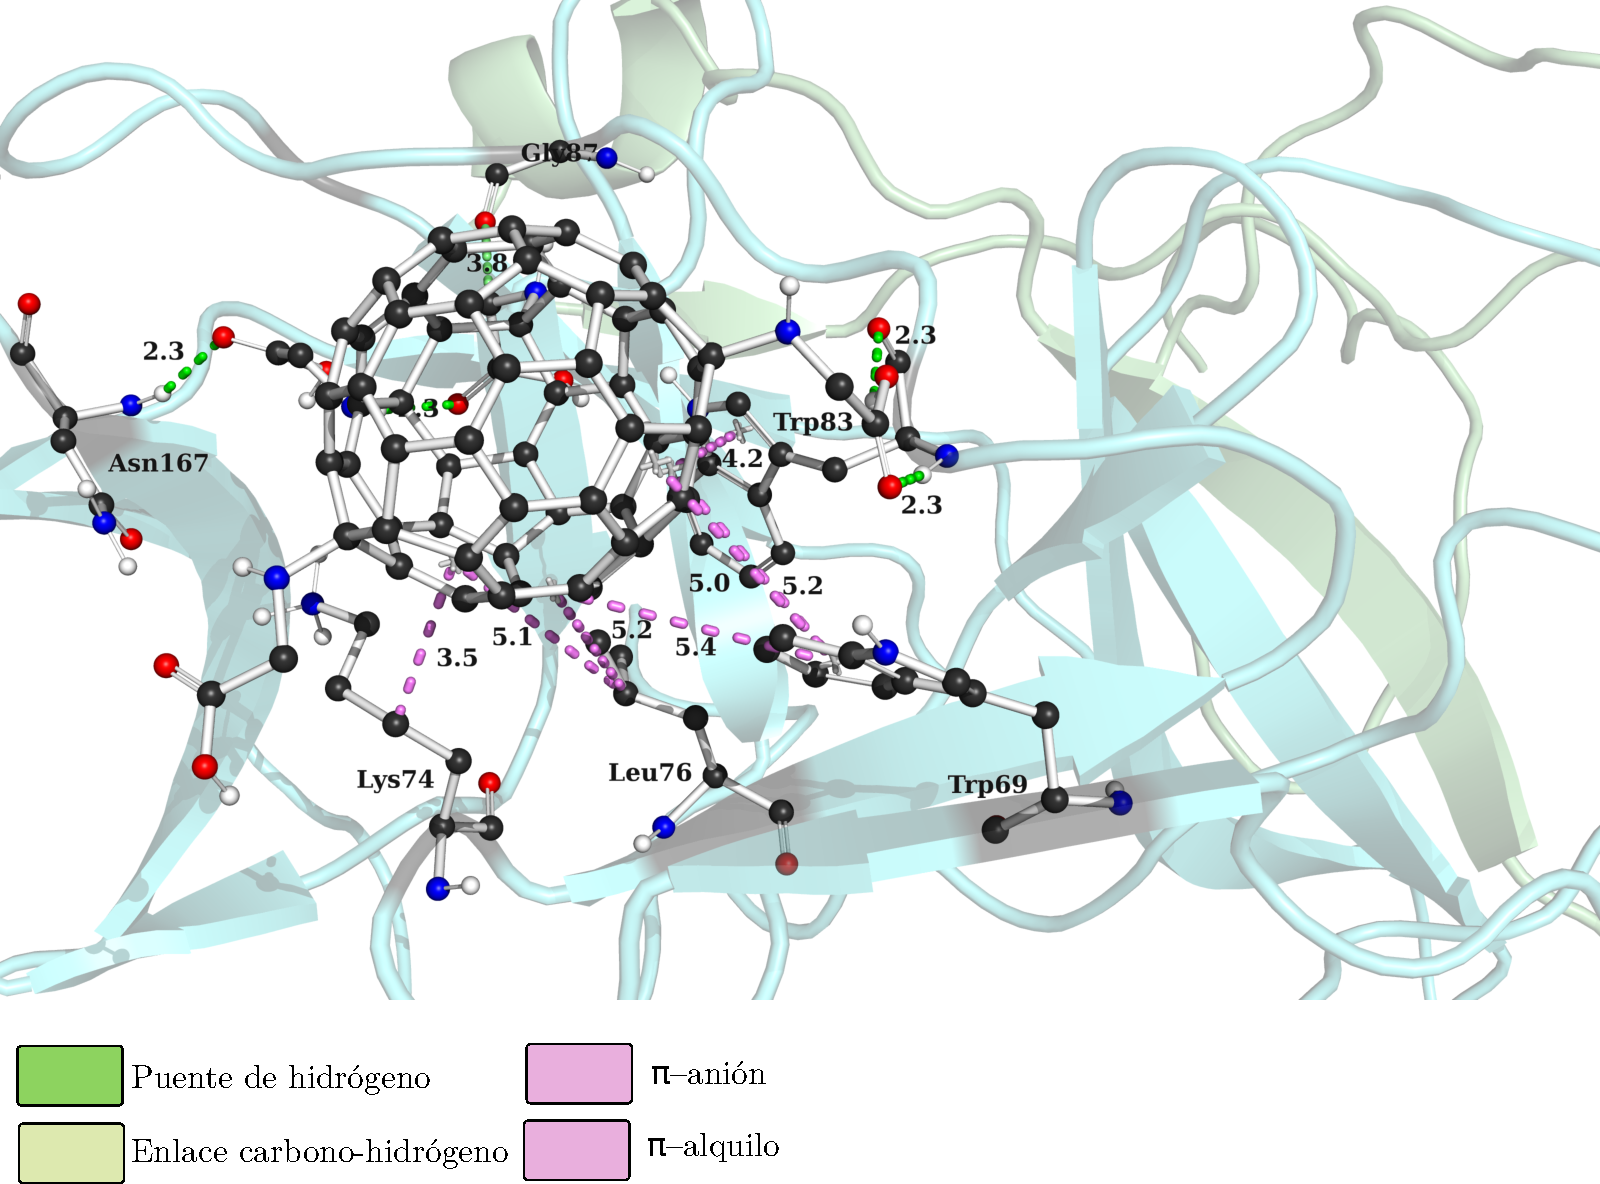
\includegraphics[width=1.0\textwidth]{imagenes/Resu/repor-c60.pdf}
      \caption{M.}
      \label{fig:mep-gly4}
        \end{figure}

\begin{figure}[H]
      \centering
      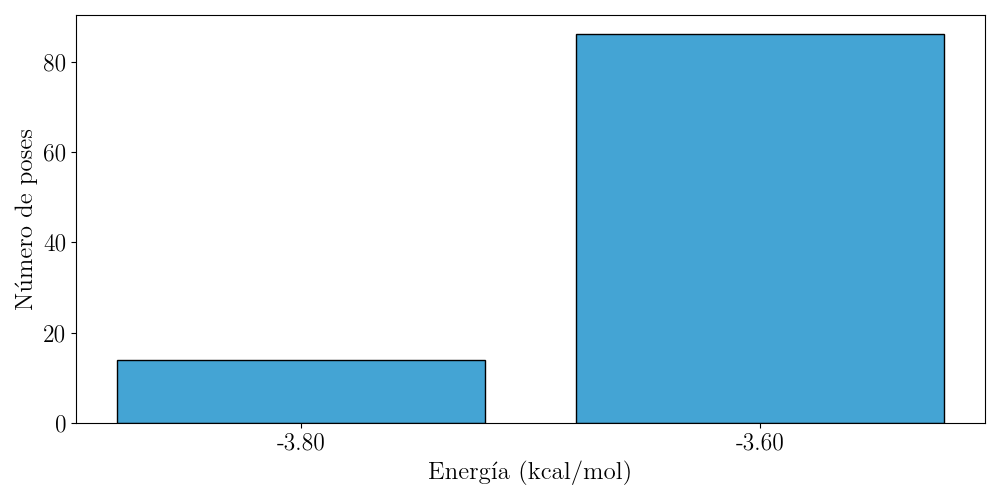
\includegraphics[width=1.0\textwidth]{imagenes/Resu/alo-resu-c60.png}
      \caption{M.}
      \label{fig:mep-gly4}
        \end{figure}
        
 \begin{table}[H]
    \centering
    \footnotesize
    \setlength{\tabcolsep}{5pt}
    \renewcommand{\arraystretch}{1.2}
    \caption{Interacciones no covalentes y distancias de contacto para el acoplamiento del derivado de fullereno C\textsubscript{60}(Gly)\textsubscript{4} en la proteasa de DENV-2 (PDB: 2FOM, Pose 61).}
    \label{tab:interacciones-pose61}
    \begin{tabular}{llcll}
        \toprule
        \multicolumn{1}{c}{\textbf{\shortstack[c]{Tipo de\\interacción}}} & 
        \multicolumn{1}{c}{\textbf{Residuo}} & 
        \multicolumn{1}{c}{\textbf{\shortstack[c]{Distancia\\(\AA)}}} & 
        \multicolumn{1}{c}{\textbf{\shortstack[c]{Motivo\\estructural}}} & 
        \multicolumn{1}{c}{\textbf{\shortstack[c]{Tipo de\\aminoácido}}} \\
        \midrule
        Puente de hidrógeno & Asn167 & 2.34 & Sitio de unión & Polar no cargado \\
                            & Trp83  & 2.32 & Bolsillo hidrofóbico & Apolar / Aromático \\
        \midrule
        Enlace de H de carbono & Gly87  & 3.67 & Sitio de unión & Apolar / Neutro \\
        \midrule
        Interacción hidrofóbica & Leu76  & 4.78 & Bolsillo hidrofóbico & Apolar / Hidrofóbico \\
        (Alquil / $\pi$-Alquil) & Trp69  & 5.22 & Bolsillo hidrofóbico & Apolar / Aromático \\
                                & Lys74  & 6.12 & Bolsillo S1 / Sitio activo & Polar, cargado positivo \\
        \bottomrule
    \end{tabular}
\end{table}       
\subsection{Evaluación del Acoplamiento Alostérico del Derivado $C_{60}(\text{Gly})_4$}

El análisis del acoplamiento molecular dirigido hacia el bolsillo alostérico de la proteasa NS2B/NS3 de DENV-2 (PDB ID: \textbf{2FOM}) se llevó a cabo bajo los mismos parámetros de exhaustividad (80) para evaluar la capacidad del aducto C\textsubscript{60}(Gly)\textsubscript{4} de actuar como un inhibidor alostérico en el sitio reportado para moléculas pequeñas como las benzamidas. A partir del muestreo de 100 poses generadas, el perfil energético (Figura~9.18) mostró una distribución conformacional altamente homogénea pero con valores de afinidad moderados: un grupo de 14 poses con una energía libre de unión de $-3.80\ \text{kcal/mol}$ y un conglomerado predominantemente mayoritario correspondiente a 86 poses con una energía de $-3.60\ \text{kcal/mol}$.

La selección de la modo de acoplamiento recayó en la \texttt{pose61.pdb}, perteneciente al grupo de mínima energía de $-3.80\ \text{kcal/mol}$. La diferencia energética entre ambos mínimos ($\Delta\Delta G = 0.20\ \text{kcal/mol}$) se encuentra holgadamente contenida dentro del margen del ruido térmico ($k_B T \approx 0.60\ \text{kcal/mol}$ a temperatura ambiente), lo que demuestra que ambas poblaciones representan microconformaciones equivalentes en rápido equilibrio termodinámico a lo largo de la entrada de la cavidad alostérica.

La caracterización visual y atómica de las interacciones no covalentes (Tabla~9.8 e Ilustración de contactos) permitió identificar el patrón de estabilización de la \texttt{pose61.pdb}:

\begin{itemize}
    \item \textbf{Puentes de hidrógeno convencionales:} Se observaron dos puentes de hidrógeno fuertes mediados por los sustituyentes de glicina del aducto con la cadena lateral de \textbf{Asn167} ($2.34\ \text{\AA}$, polar no cargado) y con el residuo aromático \textbf{Trp83} ($2.32\ \text{\AA}$), fijando las cadenas polares externas en el contorno del sitio alostérico.
    \item \textbf{Enlaces de hidrógeno de carbono (C--H):} Se identificó un contacto débil tipo $\text{C--H}\cdots\text{O/N}$ entre el esqueleto del ligando y el residuo \textbf{Gly87} a una distancia de $3.67\ \text{\AA}$.
    \item \textbf{Interacciones hidrofóbicas (Alquil / $\pi$-Alquil):} La esfera carbonosa del fulereno interacciona mediante contactos lipofílicos con los residuos \textbf{Leu76} ($4.78\ \text{\AA}$) y \textbf{Trp69} ($5.22\ \text{\AA}$) en el subbolsillo hidrofóbico, además de mantener un contacto de tipo alquilo/electrostático extendido con \textbf{Lys74} ($6.12\ \text{\AA}$).
\end{itemize}

\subsection{Análisis Comparativo entre el Derivado de Fulereno y el Inhibidor Alostérico de Referencia (Benzamida/Benzofurano)}


\begin{figure}[H]
      \centering
      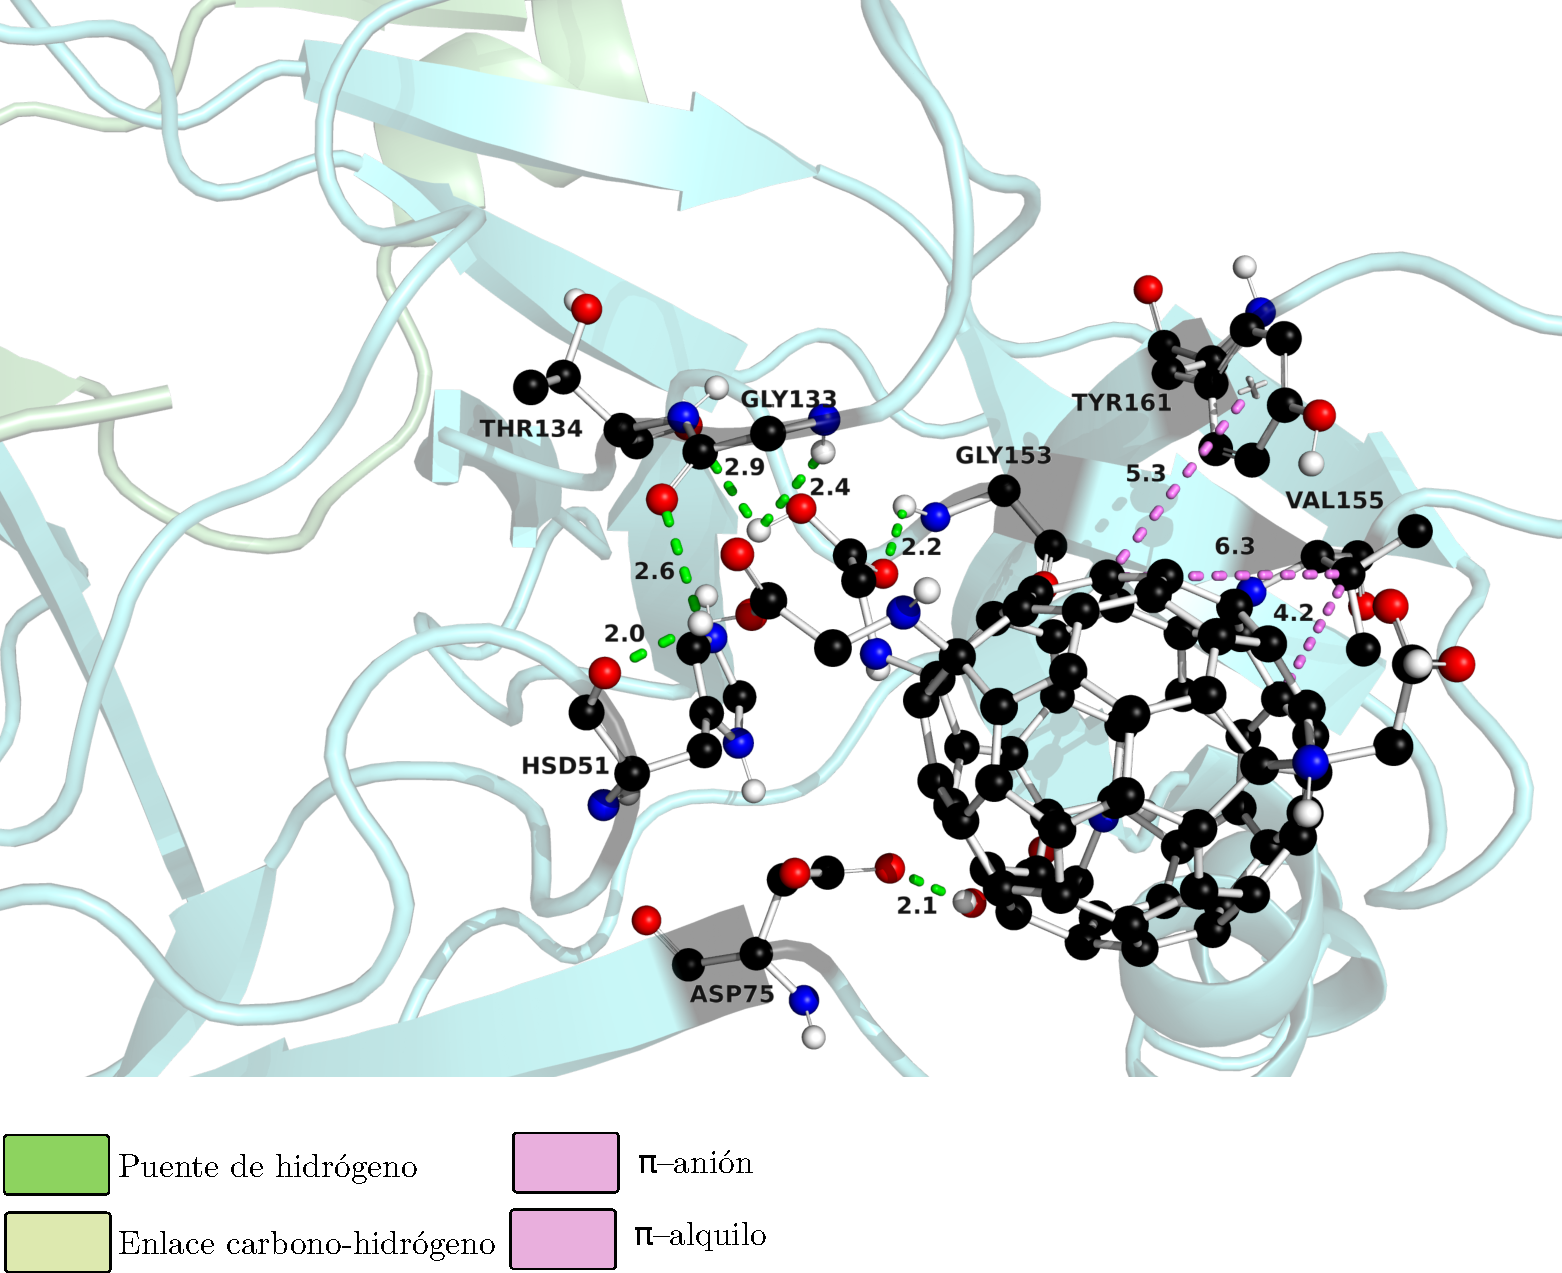
\includegraphics[width=1.0\textwidth]{imagenes/Resu/orto-1.pdf}
      \caption{M.}
      \label{fig:mep-gly4}
        \end{figure}

\begin{figure}[H]
      \centering
      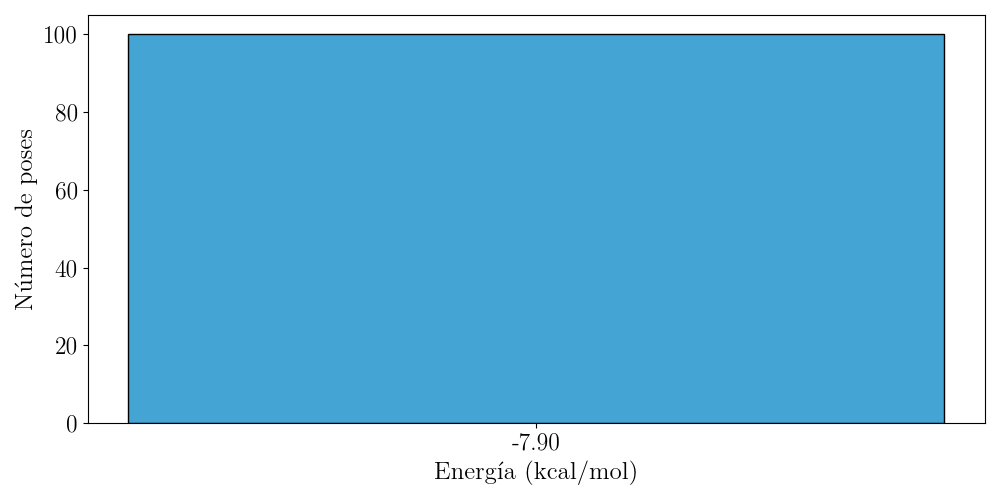
\includegraphics[width=1.0\textwidth]{imagenes/Resu/orto-c60.png}
      \caption{M.}
      \label{fig:mep-gly4}
        \end{figure}


\begin{table}[H]
    \centering
    \footnotesize
    \setlength{\tabcolsep}{5pt}
    \renewcommand{\arraystretch}{1.2}
    \caption{Interacciones no covalentes y distancias de contacto para el acoplamiento del derivado de fullereno C\textsubscript{60}(Gly)\textsubscript{4} orto-c60 en la proteasa de DENV-2 (PDB: 2FOM, Pose 1).}
    \label{tab:interacciones-pose1}
    \begin{tabular}{llcll}
        \toprule
        \multicolumn{1}{c}{\textbf{\shortstack[c]{Tipo de\\interacción}}} & 
        \multicolumn{1}{c}{\textbf{Residuo}} & 
        \multicolumn{1}{c}{\textbf{\shortstack[c]{Distancia\\(\AA)}}} & 
        \multicolumn{1}{c}{\textbf{\shortstack[c]{Motivo\\estructural}}} & 
        \multicolumn{1}{c}{\textbf{\shortstack[c]{Tipo de\\aminoácido}}} \\
        \midrule
        Puente de hidrógeno & Hsd51  & 2.05 & Tríada catalítica & Polar, cargado positivo \\
                            & Asp75  & 2.83 & Tríada catalítica & Polar, cargado negativo \\
                            & Gly133 & 2.07 & Hueco oxianiónico & Apolar / Neutro \\
                            & Thr134 & 2.63 & Sitio de unión & Polar no cargado \\
                            & Gly153 & 2.15 & Sitio de unión & Apolar / Neutro \\
        \midrule
        Interacción hidrofóbica & Val155 & 4.02 & Bolsillo hidrofóbico & Apolar / Hidrofóbico \\
        (Alquil / $\pi$-Alquil) & Tyr161 & 4.72 & Bolsillo hidrofóbico & Polar neutro / Aromático \\
                                & Tyr161 & 5.24 & Bolsillo hidrofóbico & Polar neutro / Aromático \\
        \bottomrule
    \end{tabular}
\end{table}
\subsection{Perfil Energético y Convergencia Absoluta en el Sitio Ortostérico}

El análisis del acoplamiento molecular dirigido al sitio activo ortostérico de la proteasa NS2B/NS3 del serotipo 2 del virus del dengue (PDB ID: \textbf{2FOM}) demostró una afinidad termodinámica excepcional y un patrón de reconocimiento molecular altamente específico para el aducto C\textsubscript{60}(Gly)\textsubscript{4}. A partir de una muestra de 100 poses generadas mediante AutoDock Vina (exhaustividad de 80), el perfil energético (Figura~9.20) exhibió un comportamiento conformacional extraordinario: el 100\% de las poses generadas convergieron en un único conglomerado energéticamente homogéneo con una energía libre de unión ($\Delta G$) de $-7.90\ \text{kcal/mol}$.

Esta convergencia poblacional del 100\% representa un pozo de energía potencial único y profundamente estable dentro del sitio catalítico, eliminando cualquier ambigüedad conformacional. La selección del modo de unión óptimo recayó en la \texttt{pose01.pdb} (Pose 1), la cual ejemplifica el estado en equilibrio dominante y termodinómicamente favorecido en la cavidad ortostérica.

\subsection{Análisis de Contactos No Covalentes e Interacciones Clave}

La caracterización tridimensional de las interacciones no covalentes efectuada en PyMOL y Discovery Studio Visualizer (Tabla~9.9 e Ilustración visual) permitió dilucidar la red de contactos que estabilizan el complejo nanoestructura-proteína en la \texttt{pose01.pdb}:

\begin{itemize}
    \item \textbf{Puentes de hidrógeno convencionales y anclaje catalítico:} Se identificó una densa red de puentes de hidrógeno de corta distancia ($\le 2.83\ \text{\AA}$) coordinados por las cadenas laterales del tetra-aducto de glicina:
    \begin{itemize}
        \item Interacción directa con los residuos de la tríada catalítica \textbf{Hsd51} ($2.05\ \text{\AA}$) y \textbf{Asp75} ($2.83\ \text{\AA}$), bloqueando los centros nucleofílico y de transferencia protónica de la enzima.
        \item Formación de un puente de hidrógeno fuerte con el residuo \textbf{Gly133} ($2.07\ \text{\AA}$), perteneciente al \textit{hueco oxianiónico} (\textit{oxyanion hole}), un elemento estructural crítico involucrado en la estabilización del estado de transición durante la catálisis peptídica.
        \item Contactos polares adicionales con \textbf{Gly153} ($2.15\ \text{\AA}$) y \textbf{Thr134} ($2.63\ \text{\AA}$), reforzando el posicionamiento del ligando en el contorno del sitio activo.
    \end{itemize}
    
    \item \textbf{Interacciones hidrofóbicas en el bolsillo ortostérico ($\text{Alquil} / \pi\text{-Alquil}$):} La esfera de fulereno se acomoda holgadamente en la cavidad apolar mediante interacciones de tipo $\pi$-alquilo con el residuo hidrofóbico \textbf{Val155} ($4.02\ \text{\AA}$) y contactos aromáticos dobles con la cadena lateral de \textbf{Tyr161} a distancias de $4.72\ \text{\AA}$ y $5.24\ \text{\AA}$.
\end{itemize}

\subsection{Contraste Comparativo con el Inhibidor Sintético de Referencia (246DA)}

Al comparar el desempeño del C\textsubscript{60}(Gly)\textsubscript{4} en este sitio ortostérico con el inhibidor sintético de referencia reportado en la literatura, el compuesto 246DA ($K_i = 19.84\ \mu\text{M}$ en PDB ID: \textbf{2FOM}), se identifican ventajas estructurales y bioenergéticas de gran relevancia:

\begin{enumerate}
    \item \textbf{Superioridad Energética e Incremento de Afinidad:} El aducto C\textsubscript{60}(Gly)\textsubscript{4} alcanza una energía de unión de $-7.90\ \text{kcal/mol}$, superando notoriamente la afinidad calculada para el compuesto 246DA ($-5.80\ \text{a}\ -6.00\ \text{kcal/mol}$). Esto representa una ganancia termodinámica de $\Delta\Delta G \approx -1.90\ \text{kcal/mol}$ a favorecer del derivado de fulereno, atribuible a la capacidad del núcleo de C\textsubscript{60}(Gly) de maximizar la superficie de contacto hidrofóbica en combinación con los cuatro brazos polares de glicina.
    
    \item \textbf{Conservación y Ampliación del Farmacóforo Catalítico:} Mientras que el inhibidor 246DA interactúa convencionalmente con la tríada catalítica (\textbf{His51}, \textbf{Asp75} y \textbf{Ser135}), el C\textsubscript{60}(Gly)\textsubscript{4} no solo preserva el anclaje directo con \textbf{Hsd51} ($2.05\ \text{\AA}$) y \textbf{Asp75} ($2.83\ \text{\AA}$), sino que además se ancla directamente al hueco oxianiónico (\textbf{Gly133}, $2.07\ \text{\AA}$). La oclusión simultánea de la tríada catalítica y del hueco oxianiónico sugiere un mecanismo de inhibición competitiva sumamente efectivo que previene el acceso de cualquier sustrato proteico.
    
    \item \textbf{Acomodación en el Bolsillo Lipofílico:} En lugar de la coordinación periférica observada en 246DA con residuos como \textbf{Leu76} o \textbf{Ile165}, el C\textsubscript{60}(Gly)\textsubscript{4} establece un empaquetamiento hidrofóbico optimizado mediante interacciones $\pi$-alquilo con \textbf{Val155} y \textbf{Tyr161}, validando la complementariedad volumétrica entre la cavidad y la nanoestructura esférica.
\end{enumerate}

La convergencia absoluta de las 100 poses en $-7.90\ \text{kcal/mol}$, sumada al bloqueo simultáneo de la tríada catalítica (\textbf{Hsd51}/\textbf{Asp75}) y del hueco oxianiónico (\textbf{Gly133}) a distancias $\le 2.07\ \text{\AA}$, demuestra que el derivado C\textsubscript{60}(Gly)\textsubscript{4} en la \texttt{pose01.pdb} actúa como un candidato inhibidor competitivo ortostérico de alta potencia, superando los parámetros termodinámicos del fármaco de referencia 246DA contra la proteasa del dengue serotipo 2.














